% This is a template designed by Maarten J. Waterloo for BSc and MSc
% students at the Faculty of Earth and Life Sciences, Vrije Universiteit
% Amsterdam, adapted to the University of Freiburg by Carsten F. Dormann. 

\documentclass[12pt,twoside,a4paper,final]{report}
% We define a two-side report on A-4 paper in final quality using a
% point size of 11 for the text. Other possibilities are {book},
% {article}, etc.

% A % sign indicates that text is commented out and will not appear in
% the document. Use \% if you want to indicate a % symbol in the text,
% thus 10\% will become 10%...

% We need to include some packages for layout and style. We do this
% below using the \usepackage command. A short explanation for each
% package is included.



\usepackage{amsmath}   % If you are going beyond the most basic level
                       % of displayed equations, you will benefit from
                       % using the amsmath package that plugs into
                       % LaTeX. This package has lots of useful
                       % features for multi-line equations, compound
                       % symbols, even commutative diagrams! Allows
                       % use \text in equations	

\usepackage{booktabs}  % booktabs is to enable the easy production of
                       % tables such as should appear in published
                       % scientific books and journals. What
                       % distinguishes these from plain LaTeX tables
                       % is the default use of additional space above
                       % and below rules, and rules of
                       % varying`thickness'.

\usepackage[top=3cm, bottom=3cm, outer=2.5cm, inner=3.5cm]{geometry}  
					   % formating the page margins

\usepackage{graphicx}  % The graphicx package implements LaTeX
                       % support for including graphics files,
                       % rotating parts of a page, and scaling parts
                       % of a page. The package depends on having a
                       % DVI driver that can produce these effects.
                       
\usepackage[hidelinks]{hyperref} %This package will make links in PDF
                       % documents to your figures, references, etc.
                       % hidelinks removes the boxes around the hyperreferenced items
                       
\usepackage[utf8]{inputenc} % Hard to explain: Define here the text encoding 
					   % used by your computer; on Linux typically utf8, on 
					   % windows ansinew and on mac often latin1;
					   % ideally, the whole world would use utf8
					   % important for öüäß (Umlaute)

\usepackage{palatino} % Use a nice serif font! Alternatives:
					   % times, palatino, ... 
					   
\usepackage{makeidx} % use this package to make an index
                       % of keywords, you have to follow this by the
                       % \makeindex command 
\makeindex             % Create the index file    
    
\usepackage[style=authoryear,backend=biber, maxbibnames=9,maxcitenames=1, uniquelist=false]{biblatex}

\addbibresource{reference.bib}

%\usepackage{natbib}    % Provides a style with author-year and
                       % numbered references, as well as much detailed
                       % of support for other bibliography
                       % use. Provides versions of the standard BibTeX
                       % styles that are compatible with natbib,
                       % plainnat, unsrtnat,
                       % abbrnat. The bibliography styles produced by
                       % custom-bib are designed from the start to be
                       % compatible with natbib.
                       
\usepackage{rotating}  % The rotating package implements three
                       % environments within which in-line figures,
                       % tables, and captions can be rotated by an
                       % arbitrary number of degrees. Two additional
                       % environments allow rotation of floating
                       % objects, which are typeset alone on separate
                       % pages.

\usepackage{wrapfig}   % allows text to flow around a figure               










\usepackage{tabularx}
% package for tables

% to isert R code
\usepackage{listings}
\usepackage[usenames,dvipsnames]{color}    

\lstset{ 
  language=R,                     % the language of the code
  basicstyle=\small\ttfamily, % the size of the fonts that are used for the code
  numbers=none,                   % where to put the line-numbers
  numberstyle=\tiny\color{black},  % the style that is used for the line-numbers
  stepnumber=1,                   % the step between two line-numbers. If it is 1, each line
                                  % will be numbered
  numbersep=8pt,                  % how far the line-numbers are from the code
  backgroundcolor=\color{white},  % choose the background color. You must add \usepackage{color}
  showspaces=false,               % show spaces adding particular underscores
  showstringspaces=false,         % underline spaces within strings
  showtabs=false,                 % show tabs within strings adding particular underscores
  frame=none,                   % adds a frame around the code
  rulecolor=\color{black},        % if not set, the frame-color may be changed on line-breaks within not-black text (e.g. commens (green here))
  tabsize=2,                      % sets default tabsize to 2 spaces
  captionpos=b,                   % sets the caption-position to bottom
  breaklines=true,                % sets automatic line breaking
  breakatwhitespace=false,        % sets if automatic breaks should only happen at whitespace
  keywordstyle=\color{RoyalBlue},      % keyword style
  commentstyle=\color{YellowGreen},   % comment style
  stringstyle=\color{ForestGreen}      % string literal style
}






% The \raggedbottom declaration makes all pages the height of the text
% on that page. No extra vertical space is added.
\raggedbottom

%----------------------------------------------------------------------------
% Allow more floating material on text pages:
\renewcommand\floatpagefraction{.9}%
\renewcommand\topfraction{.9}%
\renewcommand\bottomfraction{.9}%
\renewcommand\textfraction{.1}%
\setcounter{bottomnumber}{4}%
\setcounter{topnumber}{4}%
\setcounter{totalnumber}{4}%


%----------------------------------------------------------------------------
				% here the content starts !		
%----------------------------------------------------------------------------
% Define title and authors
\def\maintitle{The earthEngineGrabR - An R package to simplify the acquisition of remote sensing data}
%\def\subtitle{Subtitle...}
\def\authors{Whathave I. Learned }
\def\supervisor{Supervisor: Prof. Dr. Irene Knowitall, Department of Irreproducible Affairs}
\def\cosupervisor{Co-supervisor: Prof. Dr. Jörg Noinput, Department for the Investigation of the Unknown}
\def\year{Freiburg, May 2014}
\def\course{Bachelor thesis  (Student ID 450100) \\submitted to \\the Faculty of Environment \& Natural Resources \\ at the Albert-Ludwigs-University Freiburg}

% Start the document
\begin{document}

% Make some shortcuts for writing units and chemical species
% You can add your own here...
\newcommand{\mgl}{mg l$^{-1}$}
\newcommand{\mmoll}{mmol l$^{-1}$}
\newcommand{\meql}{meq l$^{-1}$}
\newcommand{\muscm}{$\mu$S cm$^{-1}$}
\newcommand{\water}{H$_2$O}
\newcommand{\kion}{K$^+$}
\newcommand{\naion}{Na$^+$}
\newcommand{\caion}{Ca$^{2+}$}
\newcommand{\mgion}{Mg$^{2+}$}
\newcommand{\clion}{Cl$^-$}
\newcommand{\nitrate}{NO$_3^-$}
\newcommand{\nitrite}{NO$_2^-$}
\newcommand{\nhion}{NH$_4^+$}
\newcommand{\hcoion}{HCO$_3^-$}
\newcommand{\hardness}{Ca$^{2+}$ + Mg$^{2+}$}


% Pagestyle of numbering, options are plain (Just a plain page number), empty (empty heads and feet - no page numbers), 
% headings	(puts running headings on each page), and myheadings (You specify what is to go in the heading with the 
% \markboth or the \markright commands.
% No numbering on title page, so we use empty here...
\pagestyle{empty}

%-- french title page (r) ------------------------------------------------
% Include the university-logo at the bottom of the page
\begin{figure}[h]
  \begin{flushright}
    \vspace{-2cm}
    
\includegraphics[width=4cm]{images/ufcd-logo-e1-a4-color} %ALU_longlogo}
  \end{flushright}
\end{figure}

\begin{center}
  {\huge\bfseries\maintitle\par}
  \vskip 2em%
%  {\Large\bfseries\subtitle\par}
%  \vskip 2em%
  {\Large\authors\par}
   \vskip 2cm%
  {\course\par}
  \vskip 1em%
   \begin{figure}[h]
     \begin{center}
       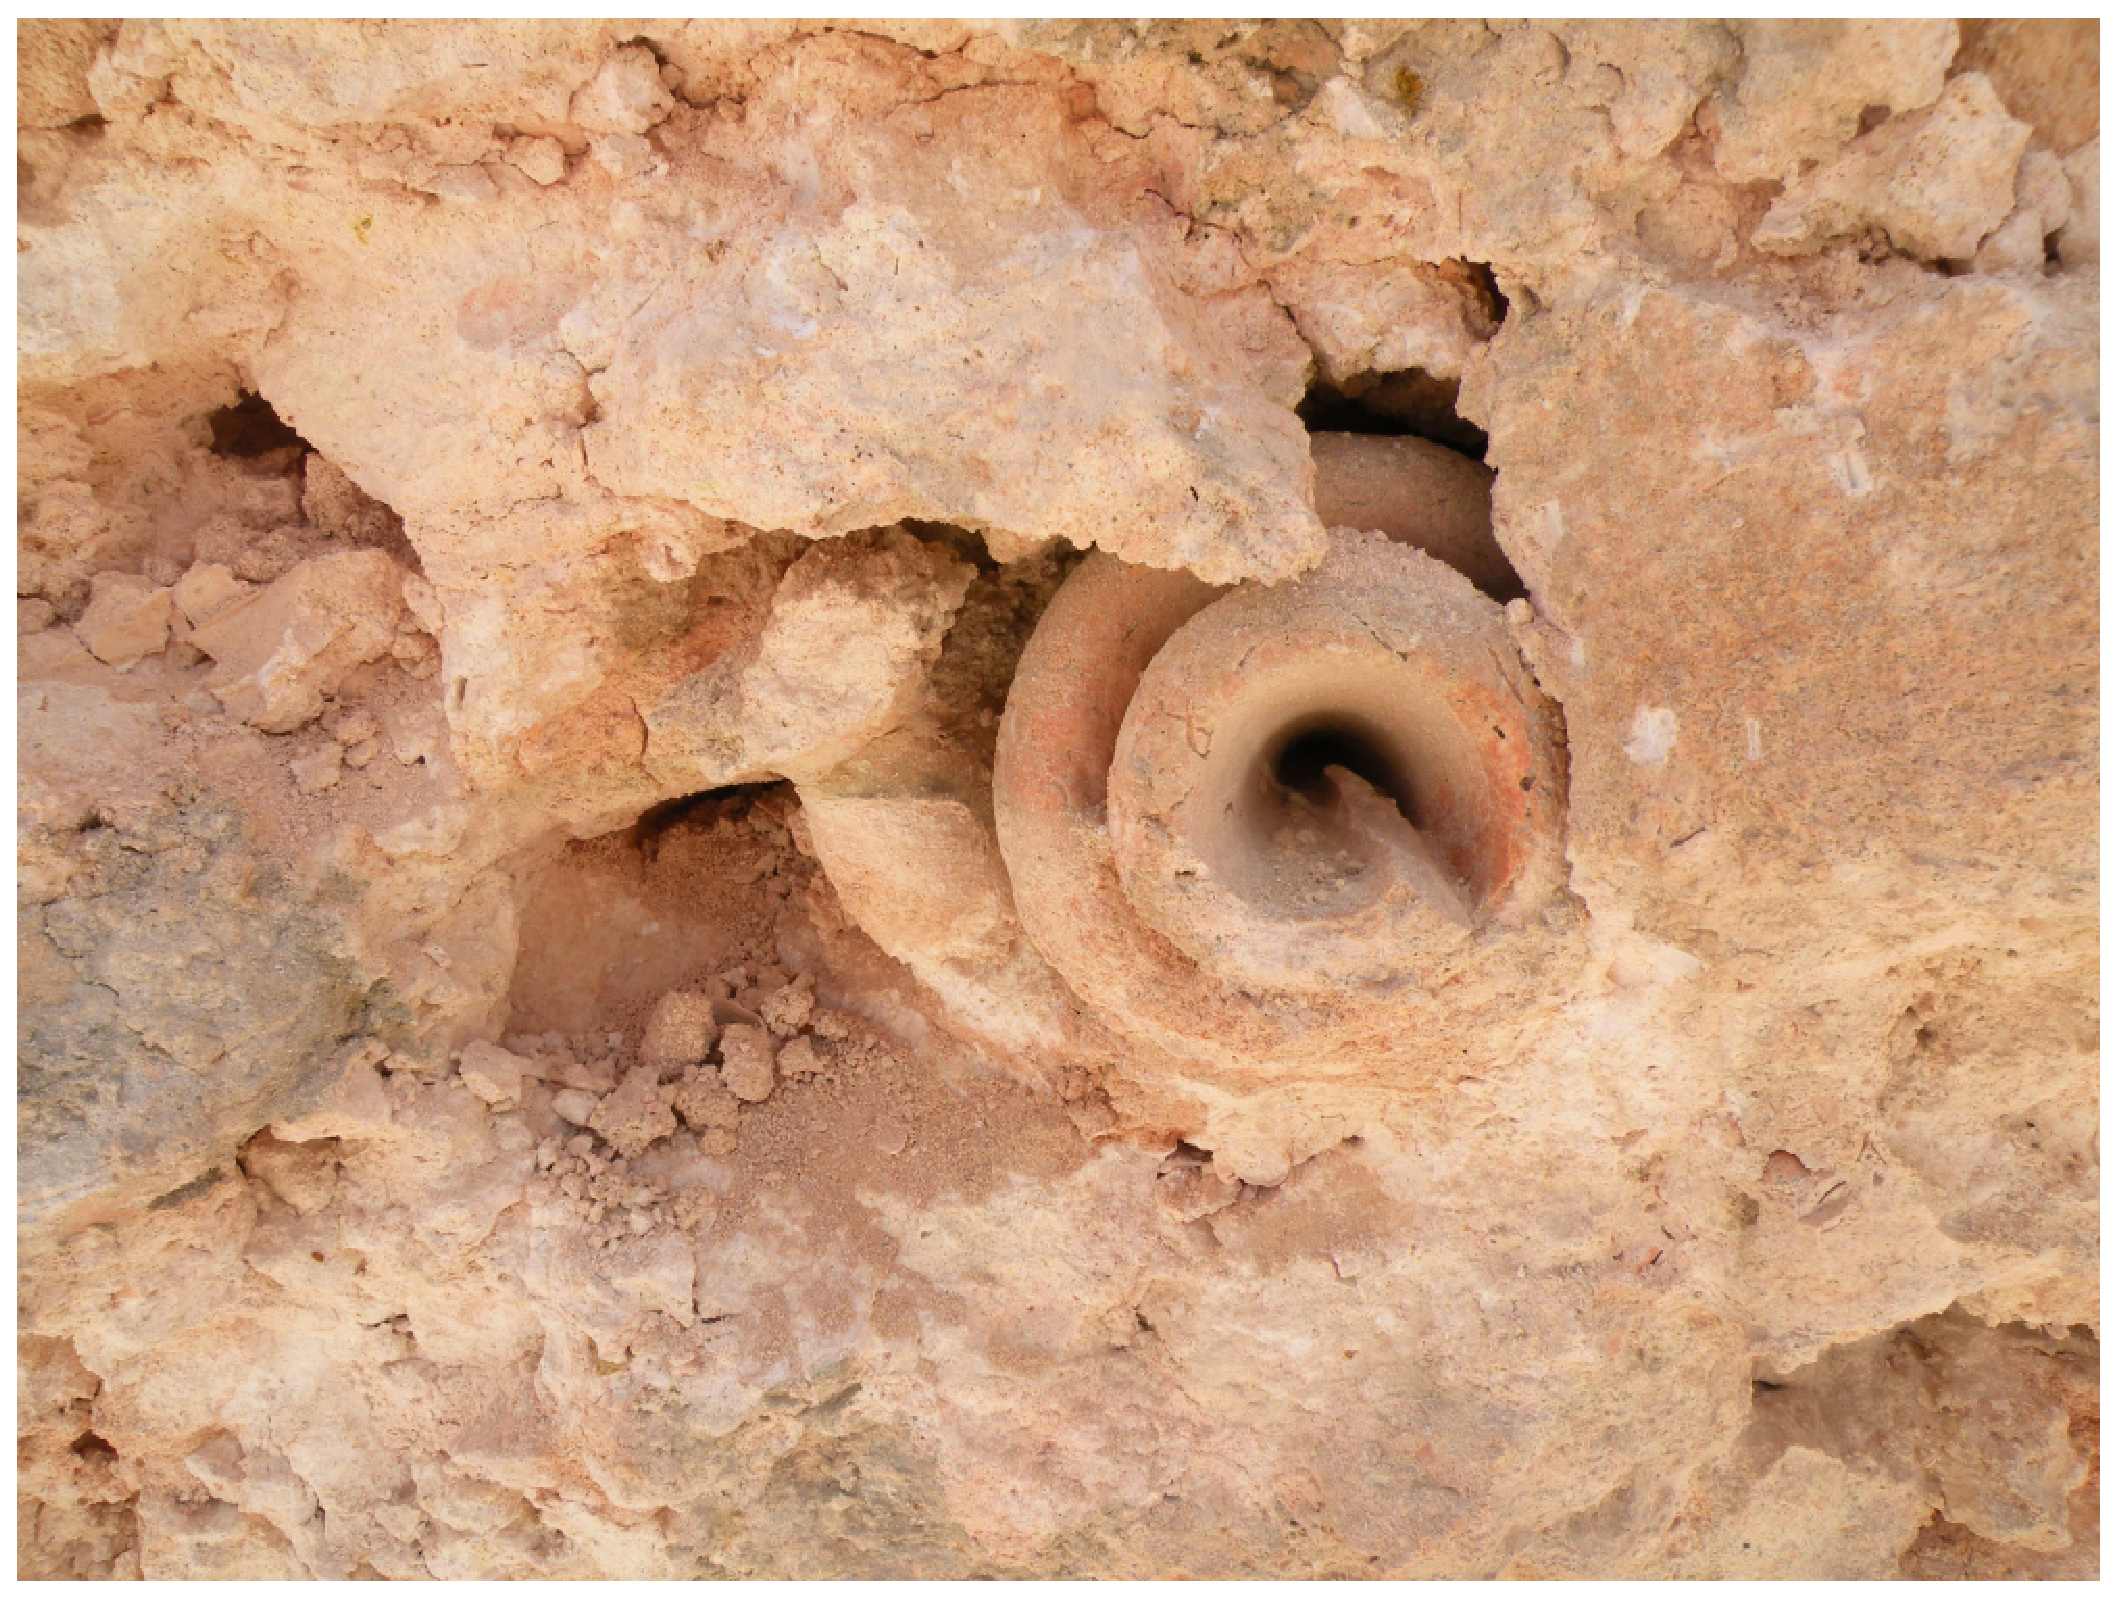
\includegraphics[width=10cm]{images/bsc-fossil}
    \end{center}
  \end{figure}
 % \vskip 2em%
\end{center}
  {\supervisor \\  \cosupervisor \\
  \flushright \year \par} 

\newpage
% If you have a photo on the titlepage, you can add a short
% explanataion here 
Cover photograph: Example of a fossil in a reef. Source: somewhere from the internet ...

\newpage

% Page numbering, options are arabic (Arabic numerals), roman	(Lowercase Roman), Roman (Uppercase Roman)
% alph (lowercase letters) and Alph (Uppercase letters)
\pagenumbering{Roman}
\pagestyle{plain}

% Include table of contents
\tableofcontents

% Remove the % in front of the command below to include a list of tables:
%\listoftables

% Remove the % in front of the command below to include a list of figures:
%\listoffigures

\newpage
% Use arabic numbering throughout the text
\pagenumbering{arabic}

% Include an abstract of your report
\abstract{

Place your abstract text here

} 
\chapter{Introduction}


To model environmental systems, information or data about the system is needed and the resources to process this data to derive insight. Remote sensing data, such as satellite imagery and derived data products, like land cover, vegetation indices, elevation models, or precipitation, are integral parts of most environmental system models. 

\section{Remote sensing data in \\ environmental system models}

The value of remotely-sensed data as a source of input data for environmental processes modelling has been increasing in the past years (\cite{melesse2007remote}). The increasing availability of remotely-sensed data from different sensors with a wide range of spatial-, temporal-  and radiometric-resolution has made remote sensing data, perhaps, the best source of data for large-scale applications for a wide range of study fields like urban studies (\cite{wu2000global}), hydrological modeling (\cite{bogh2004incorporating}), watershed mapping (\cite{melesse2003spatially}), energy and water flux estimation (\cite{melesse2005estimation}), fractional vegetation cover (\cite{carlson2000impact}) and drought predictions (\cite{rhee2010monitoring}).

Through contributions of several earth observation missions, the stock of freely available remote sensing data, as well as its temporal and spatial resolution, is continuously growing (\cite{melesse2007remote}).
However, acquiring and preparing remotely-sensed data for the use as input for an environmental system model is still related to significant expenditures of time, expertise, work and processing resources. The reason for the necessary spending is strongly related to how remotely-sensed data is acquired, stored, managed and provided.

\section{Accessibility of remote-sensing data}

Most geospatial environmental data is derived from satellite imagery. This primary satellite imagery is acquired from sensors of varies earth observation satellite missions that again are part of mainly two earth observation programmes. The most extensive programme concerning duration and the number of satellites is the Earth Observing System (EOS). The EOS is a cooperation of NASA with various Government Agencies like the National Oceanic and Atmospheric Administration (NOAA) and the United States Geological Survey (USGS), the second is the recent Copernicus Programm of the European Commission in partnership with the European Space Agency (ESA) (\cite{salomonson2002overview}). A representative satellite mission of the EOS is the Terra satellite that carries multiple sensors that among others produce the popular imagery products: Advanced Spaceborne Thermal Emission and Reflection Radiometer (ASTER) and Moderate-resolution Imaging Spectroradiometer (MODIS). The most popular satellite's mission is probably the Landsat satellites. The Copernicus Programm at the moment has two active mission: Sentinel 1 and Sentinel 2 (\cite{butler2014earth}).
From this primary satellite imagery, a multitude of secondary geospatial environmental data like Digital Elevation Models (DEMs), Land Cover, Atmosphere, Weather, Climate simulations or even socio-economic variables are derived. Examples are the National Land Cover Database (NLCD) of the USGS, the NASS Cropland Data Layers of the National Agricultural Statistics Service (USDA) but also the WorldPop project population data produced by a collaboration between researchers at different Universities worldwide (\cite{homer2007completion},\cite{johnson20102009},\cite{tatem2017worldpop}). 
With the decision of multiple U.S agencies including NASA, USGS and NOAA, as well as ESA to provide open access to their imagery data, petabyte-scale archives of geospatial data are now freely available (\cite{gorelick2017google} ).
Although freely available, all this geospatial data is separately stored in databases scattered around different governments, agencies or even universities that all have different conventions in file formats, storing or projections. 

\section{The difficulty in acquire, integrate and process remote sensing data}

Usually, the databases are accessible through an online search and order tool like the NASA Earth Observation, the USGS Earth Explorer or the Copernicus Open Access Hub. These tools allow searching for scenes of a remote sensing data product according to different metadata properties like acquisition time, name or spatial-coverage and order or download the selected scenes subsequently. 
Scenes are near-square images covering an area that varies in size depending on the remote sensing data. For Landsat images, the coverage is about 170 to 185 kilometres per scene. Because these online search and order tools do not provide any processing resource, it is not possible to aggregate or subdivide the scenes to a specific extent.

\begin{center}
	\begin{figure}[h]
		\begin{center}
			\includegraphics[width=15cm]{images/traditional_acquisition.pdf}
			\caption{Traditional method to acquire and processes remote sensing data}
			\label{traditionl_approach}
		\end{center}
	\end{figure}
	% \vskip 2em%
\end{center}


Figure \ref{traditionl_approach} shows a schematic approach of acquiring and preparing remotely-sensed data for the use as input for an environmental system model.
First, the remote sensing data must be download via one of the search and order tools. If the downloaded data is acquired from multiple sensors or different sources, the different coordinate reference systems and projections need to be integrated and harmonised. Third, in case of multiple scenes of the same locations, for instance, multiple satellite images of the same location acquired at different times, the data has to be aggregated non-spatially. For example to calculate the yearly sum of precipitation from daily chirps satellite imagery, or to calculate the NDVI from multiple bands of Landsat imagery.
Forth, the data is spatially aggregated according to a given target. The target represents the shape of the area of interest (AOI). The AOI could be a world-wide grid of 1 degree to 1-degree cells, the resolution of a raster, a set of points representing the locations of experiments, or the sample area. Finally, in the last step, the data is retrieved tabular data with a geographic reference. The entire processing of the remote sensing data was performed on the local system.
Although the order of the steps in of the workflow in Figure \ref{traditionl_approach} can vary and in some cases and specific steps can be skipped, they represent essential tasks in the acquisition and preparation of remote sensing data for environmental modelling (\cite{iosifescu2011geovite}).

Although the described method is common for the acquisition of remote sensing data for most research, the approach holds several problems and downsides.

\subsubsection{Interoperability problem}
First, because varies governments and agencies collect remote sensing data, most data is distributed and stored in different locations, in a variety of file formats, projections and resolutions. Integrate data from different sources requires a manual and thus time-consuming pre-processing of the data even when processing only a few satellite images (\cite{schell2000geodata}). To perform the required integration and harmonisation of different remote sensing data sets expertise in a geographic information system (GIS) is prerequisite.

\subsubsection{Big data problem}

Due to the limited possibility to control the request to the servers, the data throughput is unnecessary high. Even though only a fraction of a scene is needed, the complete scene needs to be downloaded. Hence, the processing resources are not where they are needed. It is required to download the entire row data to a local system to perform the tasks necessary to prepare the data for environmental modelling. The limited control over the requested data results in many unnecessary inter-products and again raises the data throughput. While processing small geospatial data sets, this may be of no importance, but for the processing of large-scale data sets, this quickly leads to challenges in dealing with memory limitation and the necessity for big data solutions like the use of computer cluster or cloud computing resources and associated challenges such as storage, management of databases and servers and managing clusters efficiently (\cite{gorelick2017google}). 
The processing of a moderately sized remote sensing imagery stack with 50 satellite images (1 Landsat-8-Collection-1-Level-1 satellite image has the size of 1.6 GB) would already require using such solutions.

\subsubsection{Restricting access}

In any case, this widely used approach to acquiring remote sensing data for environmental modelling is time consuming and resource intensive.
The time-consuming preprocessing of the data bind significant resources of processing power and expertise that otherwise could be used for the scientific work. Furthermore, although petabyte-scale archives of geospatial data are freely available, the access and utilisation of these datasets for environmental system modelling are restricted due to the given difficulties. 
These obstacles hinder most researchers to make use of this massive stack of remote sensing imagery, restricting access to the information that can be derived from large remote sensing datasets, to remote-sensing experts with exclusive access to high-performance computing resources.

The Google Earth Engine (GEE) enables much broader audience access to these resources and information.

\section{Introduction to earth engine}

Google Earth Engine is a cloud-based platform that strongly simplifies the access to high-performance computing resources to process extensive geospatial datasets, without the information technology (IT) management obstacles like, data acquisition and storage, combine different file formats, managing databases, machine allocations, CPUs, GPUs. 
Earth Engine consists of a multi-petabyte data catalogue, a high performance, parallel and therefore scaleable, computation service and is accessed and controlled through an Internet-accessible application programming interface (API).  Queries are constructed by using operations drawn from the Earth Engine client library consisting of more than 800 functions ranging from simple mathematical operations to powerful geostatistical, machine learning and image processing operations (\cite{gorelick2017google}).

\subsubsection{The data catalogue}

The majority of the Earth Engine public data catalogue consists of remote sensing imagery collected by Earth-observing satellites missions from government agencies like NASA, the US. Geological Survey, NOAA and the European Space Agency. It contains the entire archives of Landsat, Sentinel 1-2 and Modis, but also several other environmental, geophysical and social-economic datasets. This catalogue is continuously extended and updated from current missions, and this way holds up to date satellite imagery with a latency of about one day.
In Earth Engine, imagery data or raster is stored in a 2D gridded raster container referred to as an image. One image can have any number of bands, and while each band need to be homogeneous in data type, resolution and projection, bands in an image can vary in data type, resolution and projection. Each image can have associated metadata stored as key-value pairs to provide additional information like acquisition time, location or any metadata provided.
Multiple images that are related, such as images from the same source or sensor are combined in collections. These Collections provide fast spatial and temporal filtering and sorting capabilities using metadata associated to every single image in the collection. The metadata enables users to search through millions of images to select data that meet specific criteria. For example, users can quickly filter the entire Landsat 7 archive for images within Germany, collected on day-of-year 40-80, from the year 1990-2000 with cloud cover less 50\%. While this also would be possible in one of the search and order tools, Earth Engine additionally provides extensive GIS capabilities and processing resources to further manipulate the data.
For instance, the filtered Landsat scenes could be aggregated to a median composite. The bands in the median composite could be used to calculate the NDVI. The NDVI image could be spatially aggregated over multiple regions defined by the feature of a shapefile representing the state of Germany. While this process is a matter of minutes on Earth Engine, it indeed would require extended big data solutions on a local system.

What makes Earth Engine that performant is the storage system as a tile database with built-in pyramiding architecture in combination with the system architecture and several data distribution models.

\subsubsection{The tile architecture}

Images ingested into Earth Engine are preprocessed to provide fast and efficient access. First, images are parsed into tiles in the images original projection and resolution and stored in a tile database. Each tile has the size of 256 * 256 Pixels and refers to the practical trade-off between loading unneeded data vs the overhead of issuing additional reads. Instead of resampling all data to a fixed grid, traditional data cube systems would do, this method is information-preserving. Because the data is maintained in their original projection, resolution and bit depth the data degradation that is inevitable if resampling to a fixed grid, is avoided

\subsubsection{The pyramid architecture}

Additionally, a pyramid of reduced-resolution tiles is created for each image and stored in the tile database. Each level of the pyramid is produced by downsampling the previous level by a factor of two until the entire image fits into a single tile. During downsampling, continuous valued bands by default are averaged, while discrete-valued bands are aggregated using one of min, mode, max. This way, if fractions of data from an image are requested for computation in a reduced resolution, only the relevant tiles from the most appropriate pyramid level need to be retrieved from the tile database. The tile database enables Earth Engine to provide data in a variety of resolutions without introducing significant storage overhead.

\subsubsection{The system architecture}

The processing system automatically subdivides and distributes computations to enable high-throughput analysis. In Earth Engine a collection of enabling technologies is used that is available in the Google data centre environment. The Borg cluster management system is used to distribute and load-balance computation over multiple workers within a cluster. The FlumeJava framework is used for parallel pipeline execution of batch computations.
Users can interact with the Earth Engine by using either an associated web-based interactive development environment (IDE), third-party Web Apps, or directly with one of the client libraries on a local system by using the Earth Engine Python or JavaScript application programming interface (API).
The Earth Engine code editor and the third-party Web Apps use the client libraries to send requests to Earth Engine through a Representational State Transfer Application Programming Interface (REST API). 
The Tilestore Servers houses the public data catalogue in the described architecture. In the Asset Database, the user can ingest their data. 
The Borg cluster management software manages each component of the system, and each service is load-balanced over multiple workers. Failure of any individual workers results in the caller reissuing the query.

\subsubsection{Construct earth engine programmes with the client library}

The user writes Earth Engine programmes using the client library available for Python and JavaScript.
The functions in the client library can be composed to build a description of the computation the user wants to perform. This description is sent to Earth Engine servers for evaluation. To further improve performance Earth Engine uses a lazy evaluation model that allows it to compute only the fraction of output that is necessary to fulfil the current request. It postpones computing output pixels until it knows more about the context in which they are needed (\cite{gorelick2017google}).


\subsubsection{Data distribution models}

To achieve high performance, the functions in the Earth Engine library apply several built-in parallelisation and data distribution models. Each model aims to optimise a different data access pattern.
For operations that are local, image tiling is used.
In remote sensing, especially raster manipulation many processing operations are local. That is, the computation of a Pixel depends only on input pixels within a fixed distance. Examples of per-pixel operations are band math, spectral unmixing neighbourhood or convolution operations. To process operations in parallel, the area is subdivided into tiles and computed independently. This way, to process one of those tiles most of the time only a few or one input tile is needed. Image tiling combined with pyramided inputs and judicious caching provides a fast computation of results at any requested scale or projection.
For operations that are inherently non-local a spatial aggregations is used.
Non-local operations such as computations of regional or global statistics, raster-to-vector conversions, or sampling an image to train a classifier, can at least partly still be executed in parallel by aggregating together many sub-results. In Earth Engine, those processes are executed as distributed processes using a scatter-gather model. First, similar to the image tiling approach, a spatial region is divided into subregions that are allocated to workers in a distributed worker pool and computed independently. These intermediate results are sent back to the master of this computation, which combines them and transform the intermediate results into the final result. For instance, to compute a mean value each worker computes sums and counts, the master collects these intermediate results and compute the final results as the total sum by the total count.

\subsection{The potential of the GEE for the acquisition of remote sensing data}

The GEE thus offers an elegant solution for working with large remote sensing data and the related problems of the interoperability of the data due to distributed sources and the big data problems caused by the size of the data and required processing resources. 
Processing resources and data are connected, and there are no unnecessary inter-products or downloads. 
The data does not have to be download and preprocessed separately. Instead, the data is already stored one managed database, pre-processed and in access and analysis-ready format. 
The computational power required to process the data is automatically scaled, which makes computations of an entirely new magnitude possible without bothering with any information technology (IT) management obstacles.
With Earth Engine, it is possible to request and generate precisely the data needed for analysis, while any acquisition, integration, preprocessing and aggregation is outsourced to the Earth Engine servers. 

However, the GEE API is controlled by a client library, currently only available in JavaScript and Python. To use the GEE additional effort to learn and apply the client libraries is necessary furthermore, scientists using a different programming language like R cannot access the GEE API directly from within R.
There is currently no R or python package that is using earth engine capabilities to simplify the acquisition and preprocessing of remotely sensed data. Actually, there is not a single R or python package using any of earth engine capabilities directly. The few existing ones are written in python and only facilitate the use of the earth engine API by providing a pipeline to other API's like the Planet-GEE-Pipeline-GUI or provide an automated upload feature of assets via the Google Cloud Environment like the geeadd tool.

In summary, although the Earth Engine solves many of the challenges in retrieving data from large remote sensing datasets for environmental system modelling, it is still exclusive for experienced users of the Earth Engine client library available only in JavaScript and Python.

\section{The earthEngineGrabR}

To recap the current situation:
\begin{itemize}
	
	\item The stack and resolution of freely available remote sensing data, as the potential as input for environmental system model, is continuously increasing.
	\item With the traditional methods discussed, the process of acquiring remote sensing data for analysis is costly and inefficient and requires high-performance computing resources.
	\item This restricting access to the information that can be derived from large remote sensing datasets, to remote-sensing experts and deviates resources from the scientific work.
	\item The GEE provides a performant and flexible solution to the problems related to large remote sensing datasets and is superior to the traditional method of acquiring data for analysis.
	\item However, the use of the GEE is exclusive for experienced users of the Earth Engine client library only available for python.
	\item Hence, to use the potential of the GEE for the acquisition of remote sensing data, the access to the GEE needs to be simplified.
	
\end{itemize}

The simplified access to the capabilities of earth Engine would enable scientists to utilise the massive stack of freely available remote sensing data for their research projects without additional costs.

This work is inspired by the attempt to develop such simplified access to capabilities of the GEE for the R programming environment.

The Master's thesis aims to develop an R package - the earthEngineGrabR, which simplifies the acquisition of remote sensing data for the analysis in R. This should be accomplished by building an Interface between R and the GEE.
The Interface should enable to use the GEE as a backend-service to retrieve selected data sets for a given region and time of interest in an analysis-ready format. The Interface is supposed to extract data from the Earth Engine data catalogue while providing extensive control over temporal and spatial resolution. 
Any processing of the remote sensing data shall entirely be outsourced to the GEE and only the derived data products, are exported from GEE and imported in R. 

This way, the developed Interface exploits two of the GEE significant advantages. One is the public data catalogue of over 11 petabytes of remote sensing data in an analysis-ready format, and the other is its high-performance, intrinsically parallel computation service to process such massive data.

\chapter{Methods}


The GEE2R package is supposed to provide an interface of R and the GEE to acquire remote sensing data in R. The emphasis is to develop a stable framework for an interface between R and the GEE. This framework should enable the user to select from a number of data sets, choose a temporal and spatial resolution and send a request to the earth engine servers to process and export the data to the user's local machine. The framework is supposed to work as a foundation that eases further extensions.
The package consists of two functions \texttt{ee\_grab} and \texttt{ee\_grab\_init}. The \texttt{ee\_grab\_init} function handles authentications and the installation of additional dependencies necessary for the GEE2R package to work. The \texttt{ee\_grab} function retrieves the data from the GEE.

The data section:
gives an overview of the data temporarily accessible through the GEE2R package. 

GEE2R package is introduced:
dependencies and authentications handled by \texttt{ee\_grab\_init}
how the \texttt{ee\_grab} function is used to control the requested data, while the emphasis lies on the design workflow and arguments of the function.
what happens on the technical side in \texttt{ee\_grab} function call, introduce the framework for the interface of R and the GEE.

\section{Available data}
As explained earlier, the emphasis of the current version of the GEE2R package and the present thesis is to develop a stable interface of R and the GEE to retrieve data in a user-specific form. Therefore the temporally available data is still limited to a selected list of environmental variables needed in the introduction explained use case for the PhD of Severin Hauenstein...
in the further development of the GEE2R package, this list should be extended.

\begin{table}[h]
\begin{tabularx}{\textwidth}{llccc}
\hline
\textbf{data product} & \textbf{variable} & \textbf{spatial} & \textbf{temporal} & \textbf{availability}\\
\hline

MOD44B.051 & tree cover  & 30 m & yearly & 2000–2015 \\

 & non-tree cover  & 30 m & yearly & 2000–2015 \\

 & non-vegetation  & 30 m & yearly & 2000–2015 \\

JRC Global Surface Water  & Distance to surface water & 30 m & yearly & 1984–2015 \\

CHIRPS & precipitation & 0.05$^\circ$ & monthly & 2000–2015\\

SRTM & elevation  & 30 m & Single & 2000\\
 & slope  & 30 m & Single & 2000\\

Oxford MAP & Accessibility to Cities  & 0.01$^\circ$ & Single & 2015\\

& Friction Surface  & 0.01$^\circ$  & Single & 2015\\

\hline
\end{tabularx}
\caption{Datenprodukte aus dem GEE Datenkatalog}
\end{table}

Table A shows a list of environmental variables temporally accessible through the package. In the following, it is distinguished between a data product, that represents the primary source, for example, the Modis MOD44B.051 Terra Vegetation Continous Fields (VCF) and the derived environmental variable: percent tree cover.
The variables vary in temporal and spatial resolution dependent on the data product they are derived from. 
To access land cover, the MOD44B.051 Terra VCF product with a yearly temporal resolution and a 250m spatial resolution is used. The product provides a sub-pixel-level representation of surface vegetation cover, designed to continuously represent Earth's terrestrial surface as a gradient of three basic surface cover components: percent tree cover, percent non-tree cover and percent bare. The product is generated using monthly composites of Terra MODIS 250 and 500 meters Land Surface Reflectance data.
The Joint Research Center (JRC) Water Classification History is a data product, produced in collaboration with the European Commission and Google. The product provides a pixel-wise classification of surface water generated using, 3,066,102 scenes from Landsat 5, 7 and 8 acquired between 1984 and 2015. Each pixel was individually classified into water and non-water. The data comes in a basic monthly temporal resolution and an aggregated yearly resolution. In the GEE2R package, the aggregated yearly water classification product is used, providing a pixel-wise classification of seasonal water, permanent water and not water. To convert this information in a species distribution context, the data product is further processed to receive the distance to surface water for each pixel. To compute the distance permanent and seasonal water are merged, therefore the distance refers to permanent or seasonal water.

To provide topographic variables, the Shuttle Radar Topography Mission (SRTM) of NASA acquired in 2007 with a spatial resolution of 30 meters, is used. While the SRTM data product provides elevation in meters, the slope is additionally processed in earth engine. To account for Socio-economic variables the recently published Oxford MAP datasets of Accessibility to Cities for 2015 and Global Friction Surface for 2015 both with a spatial resolution of $0.01$ ($~ 30m$) are used. The global Friction Surface map estimates land-based travel speed for land pixels in the year 2015 and the global Accessibility map estimates land-based travel time to the nearest densely-populated area for the year 2015. Both datasets were produced through a collaboration between the Univerity of Oxford Malaria Atlas Project (MAP), Google, the European Union JRC. To produce the maps, the first time ever a global-scale combination of Open Street Map data and Google roads dataset was used, extended with datasets for topographic conditions, land cover types and national borders.
For the Friction Surface map, these underlying datasets were used to calculate travel speed in terms of time to cross each pixel, with the fastest travel mode intersecting the pixel being used to determine the speed to travel in that pixel. The travel speed is in minutes required to travel one meter. The Accessibility map is produced by using the Friction Surface map in combination with a least-cost-algorithm, that calculates the travel time in minutes for each pixel to the nearest city. Cities were determined by using data from the Global Human Settlement Project.  


The Climate Hazard Group InfraRed Precipitation with Station Data (CHIRPS) is a global rainfall data set with a daily temporal resolution and 0.05 spatial resolution (~150m). In the GEE2R package, the CHIRPS pentad (version 2.0 final) is utilized, an aggregated version of the daily CHIRPS dataset, with an approximately temporal resolution of 5 days.

For consistency, the data products that have a high spatial resolution like CHIRPS and JRC are only available between 2000 and 2015. This way, there is one equal time period most data is available in.

\section{organise dependencies}

organise dependencies
The GEE2R package relies on several package dependencies in R and in Python and while R dependencies for a package easily can be handled within the description file of an R package, the python dependencies need to be manually installed with a package manager like pip via the command line. Furthermore, the package connects to several APIs, which each need an individual, user-specific, authentication procedure. Therefore, a user-friendly organisation of all requirements of the GEE2R package to actually work is particularly important. To leave the installation of dependencies and authentications to the user, would greatly hinder the use of the package and make it more cumbersome. 

To solve this issue, in the GEE2R package, there is a function (\texttt{ee\_grab\_init}) that installs python dependencies and furthermore guides the user through the different authentications. Before using the GEE2R package, the user has to call \texttt{ee\_grab\_init}. The function only needs to be called once, the required authentification tokens are saved and managed independently. 
To ease the installation of the python dependencies, all dependencies are combined in a new python package (again called GEE2R), using the setuptools package in python. The GEE2R Python package can then be installed with the package manager pip. During this installation, all specified python dependencies are installed at once. This process is similar to the use of the description file in R packages. To call pip from R a system call with a command line is invoked from R. This process will be explained in details in methods for the \texttt{ee\_grab} function. 

In the GEE2R package, three APIs are used. The Google Earth Engine API, the Google Drive API and the Google Fusiontable API. Each API require an authentification with a valid Google account and in terms of the Google Earth Engine API, a Google account activated for earth engine use. According to Google, the Earth Engine is free for research, education and nonprofit use furthermore results of the analysis performed by the user, as well as new algorithms wrote by the user remain in the property of the user alone.
To get access to Earth Engine the user has to fill out a form and wait until the request for excess is granted. This activates the user's Google account to excess Earth Engine. For utilizing the Google Drive API and Google Fusiontable API only a valid Google Account is necessary. To send a valid request to one of these APIs, the request needs to be authorised with a valid access token. To manage and generate these tokens the GEE2R package uses different approaches depending on how each API is accessed. The authentification to the Google Earth Engine API is handled by the Python client library. Prior to the actual use of Earth Engine a script to generate credentials (earth engine authenticate) needs to be run. During the further use of the client library, the credentials are used to generate valid access tokens.



\section{How the data is controlled}




Instead of downloading the raw raster data the package provides control to filter and aggregate selected data products according to a given target. This processing allows retrieving the environmental variables in a specific, user-defined format. The user specifies a data product,  a time interval, a temporal reducer, a spatial reducer and a target. In the GEE a reducer is a way to aggregate data over space and time. In the GEE2R package, there are implementations for simple statistics like mean, mode, max, and min. The temporal reducer aggregates the data over time and the spatial reducer aggregates the data over a region defines by the target. 
The target is defined by a shapefile, where the spatial extent of the features define the region the spatial reducer is applied over.

\begin{center}

   \begin{figure}[h]
     \begin{center}
       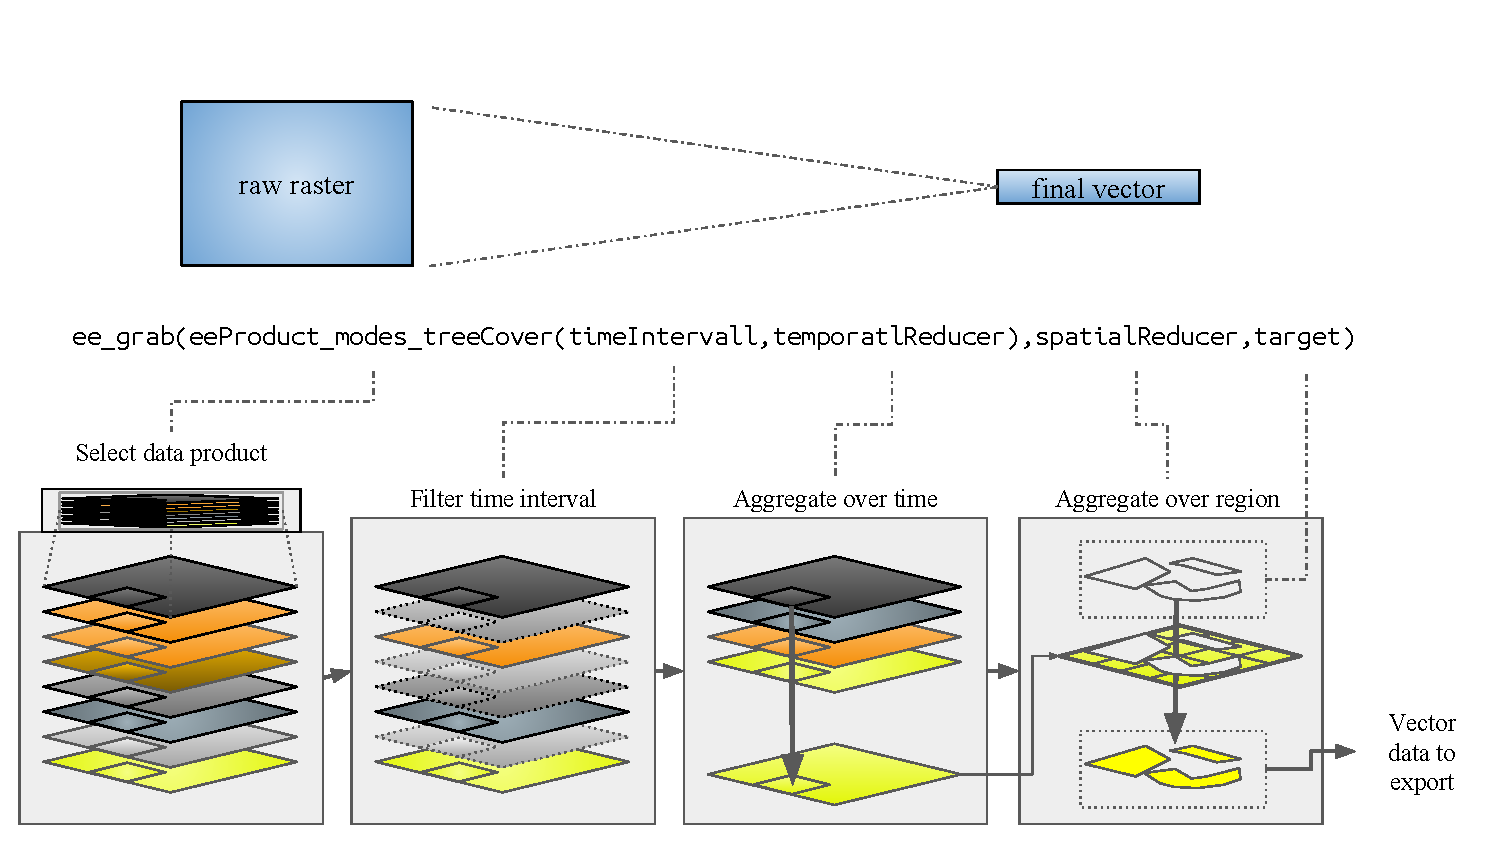
\includegraphics[width=15cm]{images/design_function.pdf}
    \end{center}
  \end{figure}
 % \vskip 2em%
\end{center}

Image 1 shows the basic processing flow to retrieve an environmental variable in a defined format. First, the data product is selected, if the data has a temporal resolution, the time interval is used to filter the data. The images passing the filter are reduced to one image with the given temporal reducer. Next, for each region of the raster overlapping with a feature in the target shapefile a reducer is applied and a statistic is computed. The output of this process is a feature collection in the vector format. This feature collection is exported to the user's local machine.
During this entire processing flow, the size of the data is massively reduced. All 



\section{technical structure}

To enable R users to request and download data from the GEE, the package combines multiple tools like the programming languages R, Python, as well as multiple web services provided by Google like the Fusion Tables, Google Drive and of course the GEE. While Google Drive is a general file sharing and storage service for all kinds of files, Google Fusion Table is specifically designed to manage tabular data and enables to upload, manipulate, visualize and share small amounts of data online.
 
Each tool performs a specific task. In R, the user specifies the requested data and initializes all further processes. In Python, the actual request is generated and send to the GEE. Because the GEE can import Fusion Tables, the Google Fusion Table is used to upload local vector data to the GEE. The GEE performs all data processing and exports the data to Google Drive wherefrom it's downloaded and imported into R. 


\begin{center}

   \begin{figure}[h]
     \begin{center}
       \includegraphics[width=15cm]{images/processin_folw.pdf}
    \end{center}
  \end{figure}
 % \vskip 2em%
\end{center}

Flowchart A shows a schematic sequence of processes that are executed in the main \texttt{ee\_grab} function call. The Flowchart is divided between processes that are performed locally and processes performed by some kind of web server on the cloud. On the local machine, the black box illustrates the function call in the R console while the 3 main folders correspond to the GEE2R library folder, the temporal working directory and the folder for the earth engine python client library. The folders contain two different sorts of files, either the bright R or Python scripts, that execute specific tasks or the dark data files that stands for intermediate products in the processing chain.
At the beginning of the function call, the target vector data is uploaded as Fusion Table illustrated with the dark yellow arrows with number 1. 
The group of processes with the number 2 in red, describes the integration of R and Python and the way python code is executed from R. The processes with number 3 in yellow, represents the exchange of arguments, or,  how parameters are passed from R to Python. The orange arrows with the number 4 illustrate the structure of the python code as executable modules. The blue processes with the number 5 show the communication of the python client library and the GEE while the dark blue arrows with number 6 describe the approach to send process info from GEE to R. In dark grey with number 7 the import of the Fusion Table the computation and the export of the processed data is illustrated and finally the green processes with number 8, describes the access from R to Google Drive and the following download and import of the final data into R.
Based on the classification of the flowchart, the following section explains all 8 groups of processes in detail.

If installed, the GEE2R R library is located in a default library folder for all R libraries. In the GEE2R folder, there is R folder, containing an R script, which defines all R functions used in the package. Furthermore, there is an additional Python folder containing python scripts divided into execution scripts and function scripts. The function script, again, defines all python functions. The execution script, however, is executed from R and uses these functions.

To upload the target vector data the Fusion Table driver in the Geospatial Data Abstraction (GDAL) library is used. To execute GDAL from R, R's ability to invoke function calls is applied, this method will be explained in more detail in the following section. The upload process is handled by GDAL's ogr2ogr function, that converts a variety of geo file formats to a Fusion Table. In Fusion Tables, geometries need to be expressed in the World Geodetic System 1984 (WGS84). Therefore the projection of the geodata uploaded as Fusion Table is converted and if necessary needs to be reprojected in earth engine.
The GEE is accessed with the GEE client library available for python. To access the GEE from R it's necessary to execute python from R. The integration should enable to pass arguments from R to Python and execute Python code from R. Instead of using a python wrapper for R like the rPython package, GEE2R utilizes a simple command line or terminal to execute one language from the other, illustrated by the red arrows with the number 1. The \texttt{ee\_grab} function defined in the R script functions.R, in red, invokes a system call by utilizing the command line that executes the python execution script (execution.py) and simultaneously, in yellow with the number 2, passes the parameters, to the execution scripts by using a flat file. 

\begin{center}

   \begin{figure}[h]
     \begin{center}
       \includegraphics[width=15cm]{images/concole_connection.pdf}
    \end{center}
  \end{figure}
 % \vskip 2em%
\end{center}


To show this two processes in practice, image B shows a simplified code example of how to retrieve metadata of a specified data product from the GEE in R with the command line as the connection of R and python. The image presents how to execute python code from R in red and how to pass parameters from R to Python in yellow. The left boxes illustrate the R console, the right box the Python execution script and the black box the command line.
In R the system2 function of the base package invoices system commands and additional arguments in all operating systems. 
To run the python script \texttt{get\_info.py} the system call simply consists of the command \texttt{python}, to open the python interpreter and the path to the python script. The system2 function then produces the system call in the command line shown in the black box and runs the \texttt{get\_info.py} script. To pass parameters from R to Python a flat file connection is used. The Parameter is defined in R, then written to a CSV file and read again into the execution script. In this example, the parameter is the asset-id of the Shuttle Radar Topography Mission (SRTM) in the GEE. 
In the Python script \texttt{get\_info\_execution.py}, first the earth engine client library is imported and initialized with the authentication credentials then the parameters are imported. To load the SRTM data product from the GEE data catalogue the asset-id is put inside an earth engine object (\texttt{ee.Image()}) specifying an image. To access metadata from this earth engine object their getInfo method is called and put inside a print statement. The output of this script is the output of the print statement. This output is formatted in JSON and in the default setting of the system2 function directly printed to the R console. Although simplified, this example shows the basic integration of R and Python and the way to send parameters. 

\subsubsection{sending parameters}

Although it would be possible to send parameters directly over the command line, with an increasing number of parameter, this method becomes confusing and error-prone due to text formatting differences of the command line dependent on the operating system. Therefore the package utilizes a flat file connection that provides a reliable method to exchange parameters independent from the operating system.

\subsubsection{organize python code os modules}

All necessary processing of the data in the GEE is described with the ee client library in python. To maintain a well-arranged structure the code is organised like a sub-package, inside the GEE2R package. There is an execution script, executed with the method described above, that calls functions defined in a python script (functions.py). This relationship is illustrated in image (full) with the orange arrows with number 3, that appears as a circle. This python script defines all functions necessary for the data processing chain shown in Image (data processing chain). The functions are organised like independent modules, each describing one process in the processing chain shown in (data processing chain). This causes functions for temporal filtering and reduction, spatial reduction and export. The modules take the parameters as function arguments and this way provide the described control over the requested data (method introduction).

\subsubsection{use of the client library}

The client library consists of Objects, that represent placeholders for datatypes stored on the earth engine servers, each object has corresponding methods or functions that manipulate this data type. Image (code example) shows an example of an earth engine object for an Image. To perform a computation in earth engine, the objects and corresponding methods are composed and combined,  building a description of the computation the user wants to perform. 

\subsubsection{communication of client library and earth engine}

At the moment the script is executed, this description is sent to the earth engine servers, in image X indicated as blue arrow with the number 4, through a Representational State Transfer Application Programming Interface (REST API). REST is a web service often used to request and modify data on a server through a Hypertext Transfer Protocol (HTTP).
In the context of the earth engine client library, it refers to using HTTP verbs to retrieve and modify representations of data stored by Google.
In a REST system, resources are stored in a data store. A client sends a request that the server performs a particular action (such as creating, retrieving, updating, or deleting a resource), and the server performs the action and sends a response. In the case of the GEE2R package, the request is: import a specific data product, filter time interval, aggregate over time, aggregate over regions and export the generated data to Google Drive (see data control and imageX dark grey arrow with number 6). While this is the action of the request that is performed the response of the request is to send info about the export process, in image X represented as a dark blue arrow with number 5. This process info includes metadata of the exported object and whether the export was successful or not. To send this info to R again a flat file connection is used, because the response is in JavaScript Object Notation (JSON), the info is written to disk as a JSON file and afterward imported into R. The last step in the processing chain is to access Google Drive from R and first Download and after Import the data into R in image X shown as green arrows with number 7. To access Google Drive from R the "googledrive" R package is used. The googledrive package enables selection and download of specific files stored on the users Google Drive account. To identify the files to download, the metadata included in the retrieved process info is used. First, the data is downloaded in the temp folder and if available on disk imported into R.


\chapter{Results}

\section{example situation 1}

You are a scientist involved with the MIKE Programm (Monitoring the Illegal Killing of Elephants). Your object of investigation is to find covariates for the intensity of illegally killed elephants in Africa. You have access to data collected within the Great Elephant Census, a continent-wide aerial survey counting the number and distribution of elephants within there territories. 
Image X shows the study area, each region corresponds to a territory and for each territory, you have the aggregated number of illegally killed elephants. To run your statistical model in R and find influential covariates you need further environmental variables derived from satellite imagery like the topography, land-use, precipitation et cetera. 
Although the study area is fragmented and of large-scale at the same time to acquire the data with the GEE2R package is pretty convenient.
The study area is fragmented and of large-scale at the same time. 
data product
After installing the GEE2R package the first step is to initialize the package with \texttt{ee\_grab\_init()}. As described in the section (methods dependencies) the function installs all additionally required dependencies and guides the user through the authentication processes to activate the different API's. To authenticate to the API the user has to log in to his Google account and allow the API to access data on googles servers on the user's behalf. If the Google account is verified and the permission is granted, the user is directed to an authentification token. This token is manually copied and pasted into a running command line script, which creates persistent credentials. 
Later, the credentials are used to authenticate a request to the API. To simplify this procedure the \texttt{ee\_grab\_init()} function successively opens a browser window to log into the Google account and a corresponding command line window to enter the token. This process is repeated for each API. If the function runs successfully, all needed credentials are stored for further sessions. Because some of the credentials expire after a few hours, a reauthentication is necessary. This process is handled automatically inside the \texttt{ee\_grab()} function. If a reauthentication is needed the function opens a browser window and the user is asked to log in with his google account, the creation of credentials is automated and there is no need to copy or paste the token manually.
To acquire the data next the \texttt{ee\_grab()} function is used.

\begin{center}

   \begin{figure}[h]
     \begin{center}
       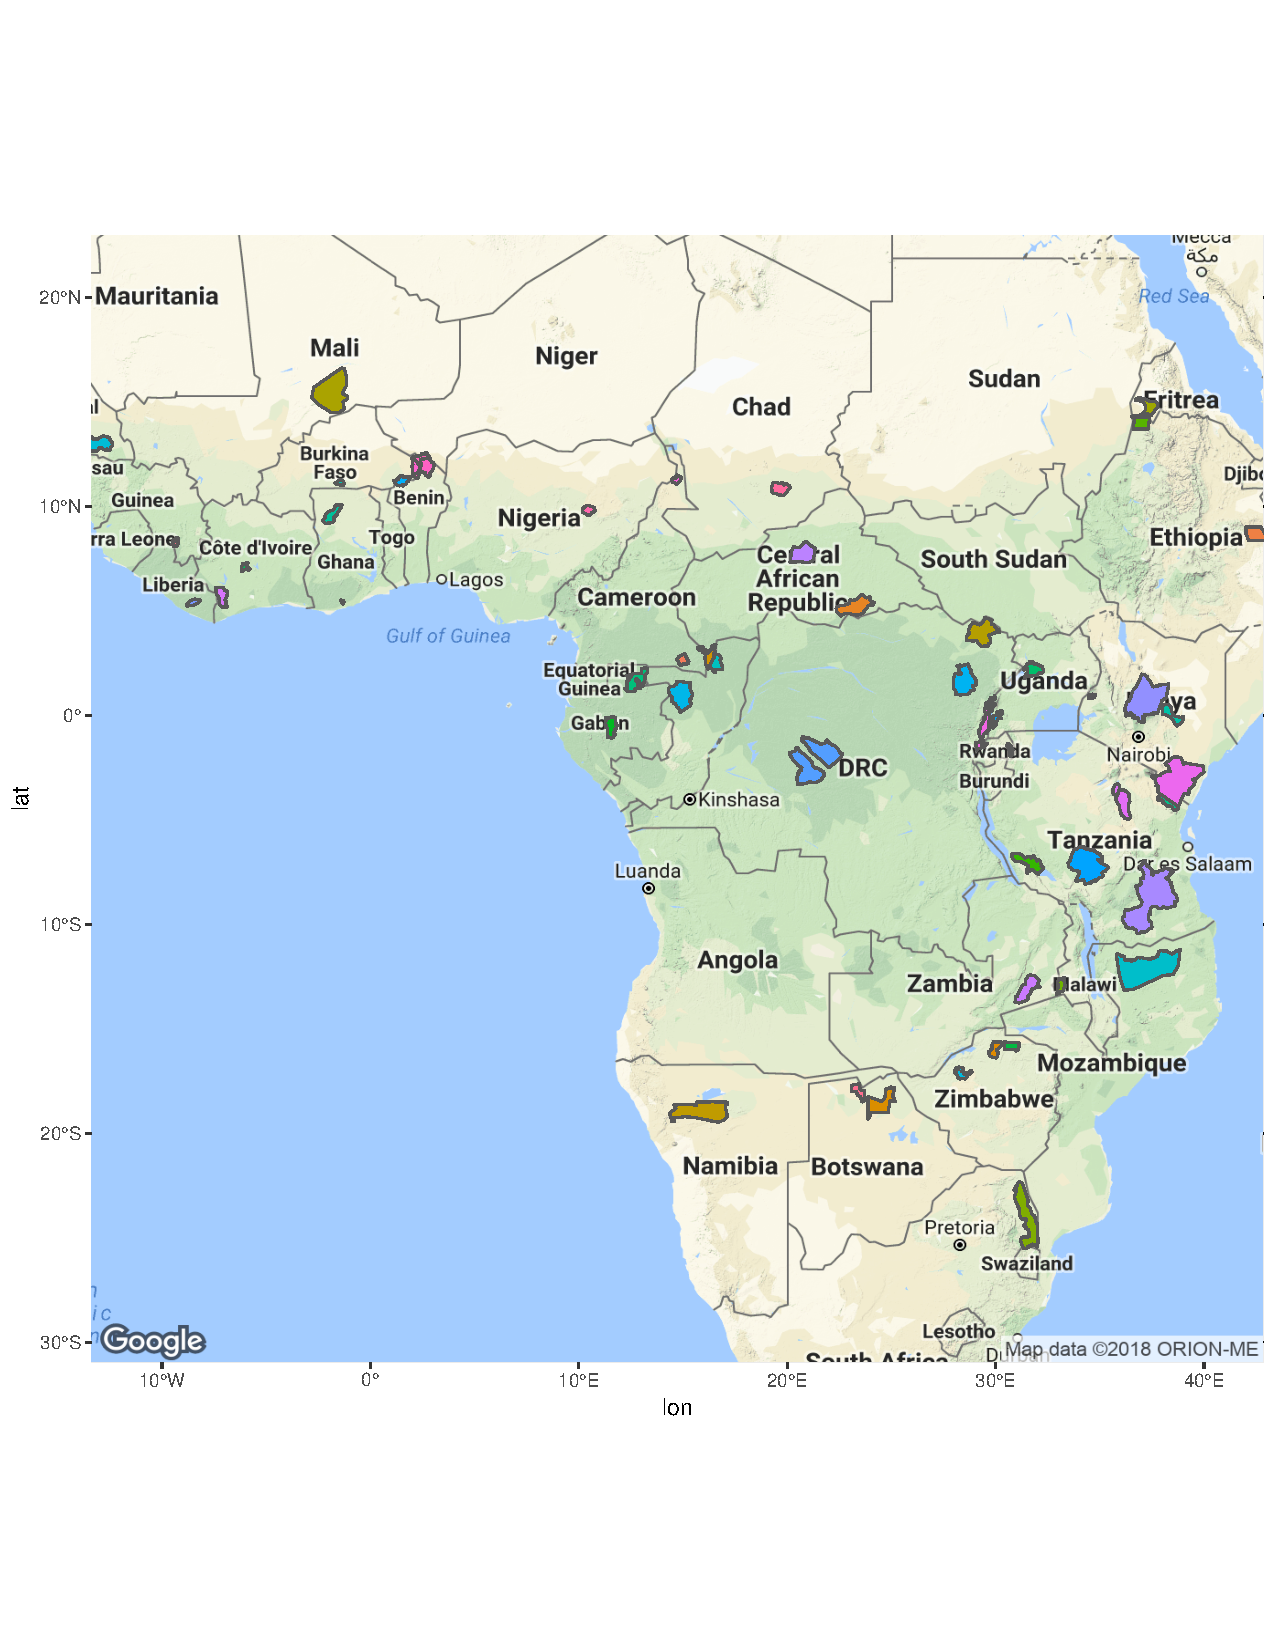
\includegraphics[width=15cm]{images/territories.pdf}
    \end{center}
  \end{figure}
 % \vskip 2em%
\end{center}

The target is the path to the shapefile of the elephant territories shown in image X. The products argument takes a list of earth engine data product-functions. Each function specifies one particular data product and it's necessary parameter. The name of the function is \texttt{eeProduct\_ }followed by the source of the data products, underscore the name of the data product. For example: \texttt{eeProduct\_modis\_treecover()}. The output of the function is simply an Object of class list, that specifies the parameters of the requested data product. To use a function, that produces the required parameters instead of committing a list or a vector with the listed parameter, holds several advantages. Because all data products start with \texttt{eeProduct\_ }, by simply typing \texttt{eeProduct\_ }, R's autocomplete function opens a drop-down menu of all available data products. Furthermore, the selection of a product in the menu displays a little description of the product and list their possible parameters. For more Information on a particular data product simply open the documentation of the function by pressing F1, or use equivalent methods. This way, it's possible to browse through the products, without any additional metadata outside of R. Additionally the functions provide default parameter values, that allow a test run without the need of specifying any parameter. While this procedure provides a user-friendly selection of available data products with their corresponding parameters it also minimises potential typing and spelling errors.
After browsing through the data products you choose the modis-tree-cover product for the year 2000 to 2005. You are further interested in the mean tree cover between this period and also want the mean tree cover in each of your territories. Because the default value for the time reducer and the spatial reducer is mean you only need to specify the time interval parameter with a vector of the start and end-year (\texttt{timeInterval = c(2000, 2005)}). You are further interested in a potential correlation of the accessibility to populated areas and the illegally killed elephant, therefore you additionally choose the oxford-accessibility product. The information displayed by the R's autocompleting feature reveals only one possible parameter - spatialReducer - and by requesting the documentation of the function you learn that this data product is only available for the year 2015, and therefore has no temporal resolution to aggregate. Again, you choose the mean accessibility in each territory by using the default value of the parameter and add the function product to the list. The last argument specifies is the resolution in meters (edge length). The resolution sets the resolution of the processed data in Earth Engine and applies for all products. A value smaller than the native resolution of the data product results in Earth Engine resampling the data with the default nearest neighbour method, values higher result in a pixel aggregation with a default method mean. In the documentation, you learned that the native resolution of the tree cover product is 250m while the accessibility products provide a resolution of 30m. Because the area of the territories is of large-scale (mean area of the territories is 9862 square kilometres) you choose 1000m as the scale of your analysis. The resolution parameter strongly controls the scope of computation and out of this the processing time, therefore it's a good choice to not unnecessarily set him too low. 
Since all parameters are set, the function can be executed. 

\begin{lstlisting}
library(earthEngineGrabR)

ee_grab_init()


africa_elephant_data <- ee_grab(
  target = "../Data/drought_sites/mike_bnd_af.shp",
  products = list(
    eeProduct_modis_treeCover(yearIntervall = c(2008, 2012)),
    eeProduct_oxford_accessibility()
  ),
  resolution = 1000
)
\end{lstlisting}


As most processes of the function call are processed on googles servers, the execution time depends strongly on the throughput of your analysis on the servers and only slightly on the performance of your local machine. However, because of the upload and download process during the function execution, very low internet speed (1 Mbit/s in download and 0.1 Mbit/s in upload) can work as a bottleneck, particularly during the upload process. 
On a 64 bit ubuntu machine with 8 Gbit RAM, 4 cores with 2.40GHz and internet speed of $10 \frac{Mbit}{s}$ in download and $1 \frac{Mbit}{s}$ in upload the \texttt{ee\_grab } function took 55 seconds to execute. All further time measurements refer to this setting.
The output of the \texttt{ee\_grab} function is an object of class "sf". The "sf" package provides a convenient approach to work with vector data in R and tries to succeed the widely used "sp" package in the future. For further information about the "sf" package see (). An "sf" object is basically a data.frame with an additional geometry list-column, what strongly simplifies manipulating an "sf" object by filtering, selecting or summarising.  The output of the \texttt{ee\_grab} function always contains all properties of the original target with the added products. The object new produced columns for the data products and a geometry column (see table X).


\begin{center}

   \begin{figure}[h]
     \begin{center}
       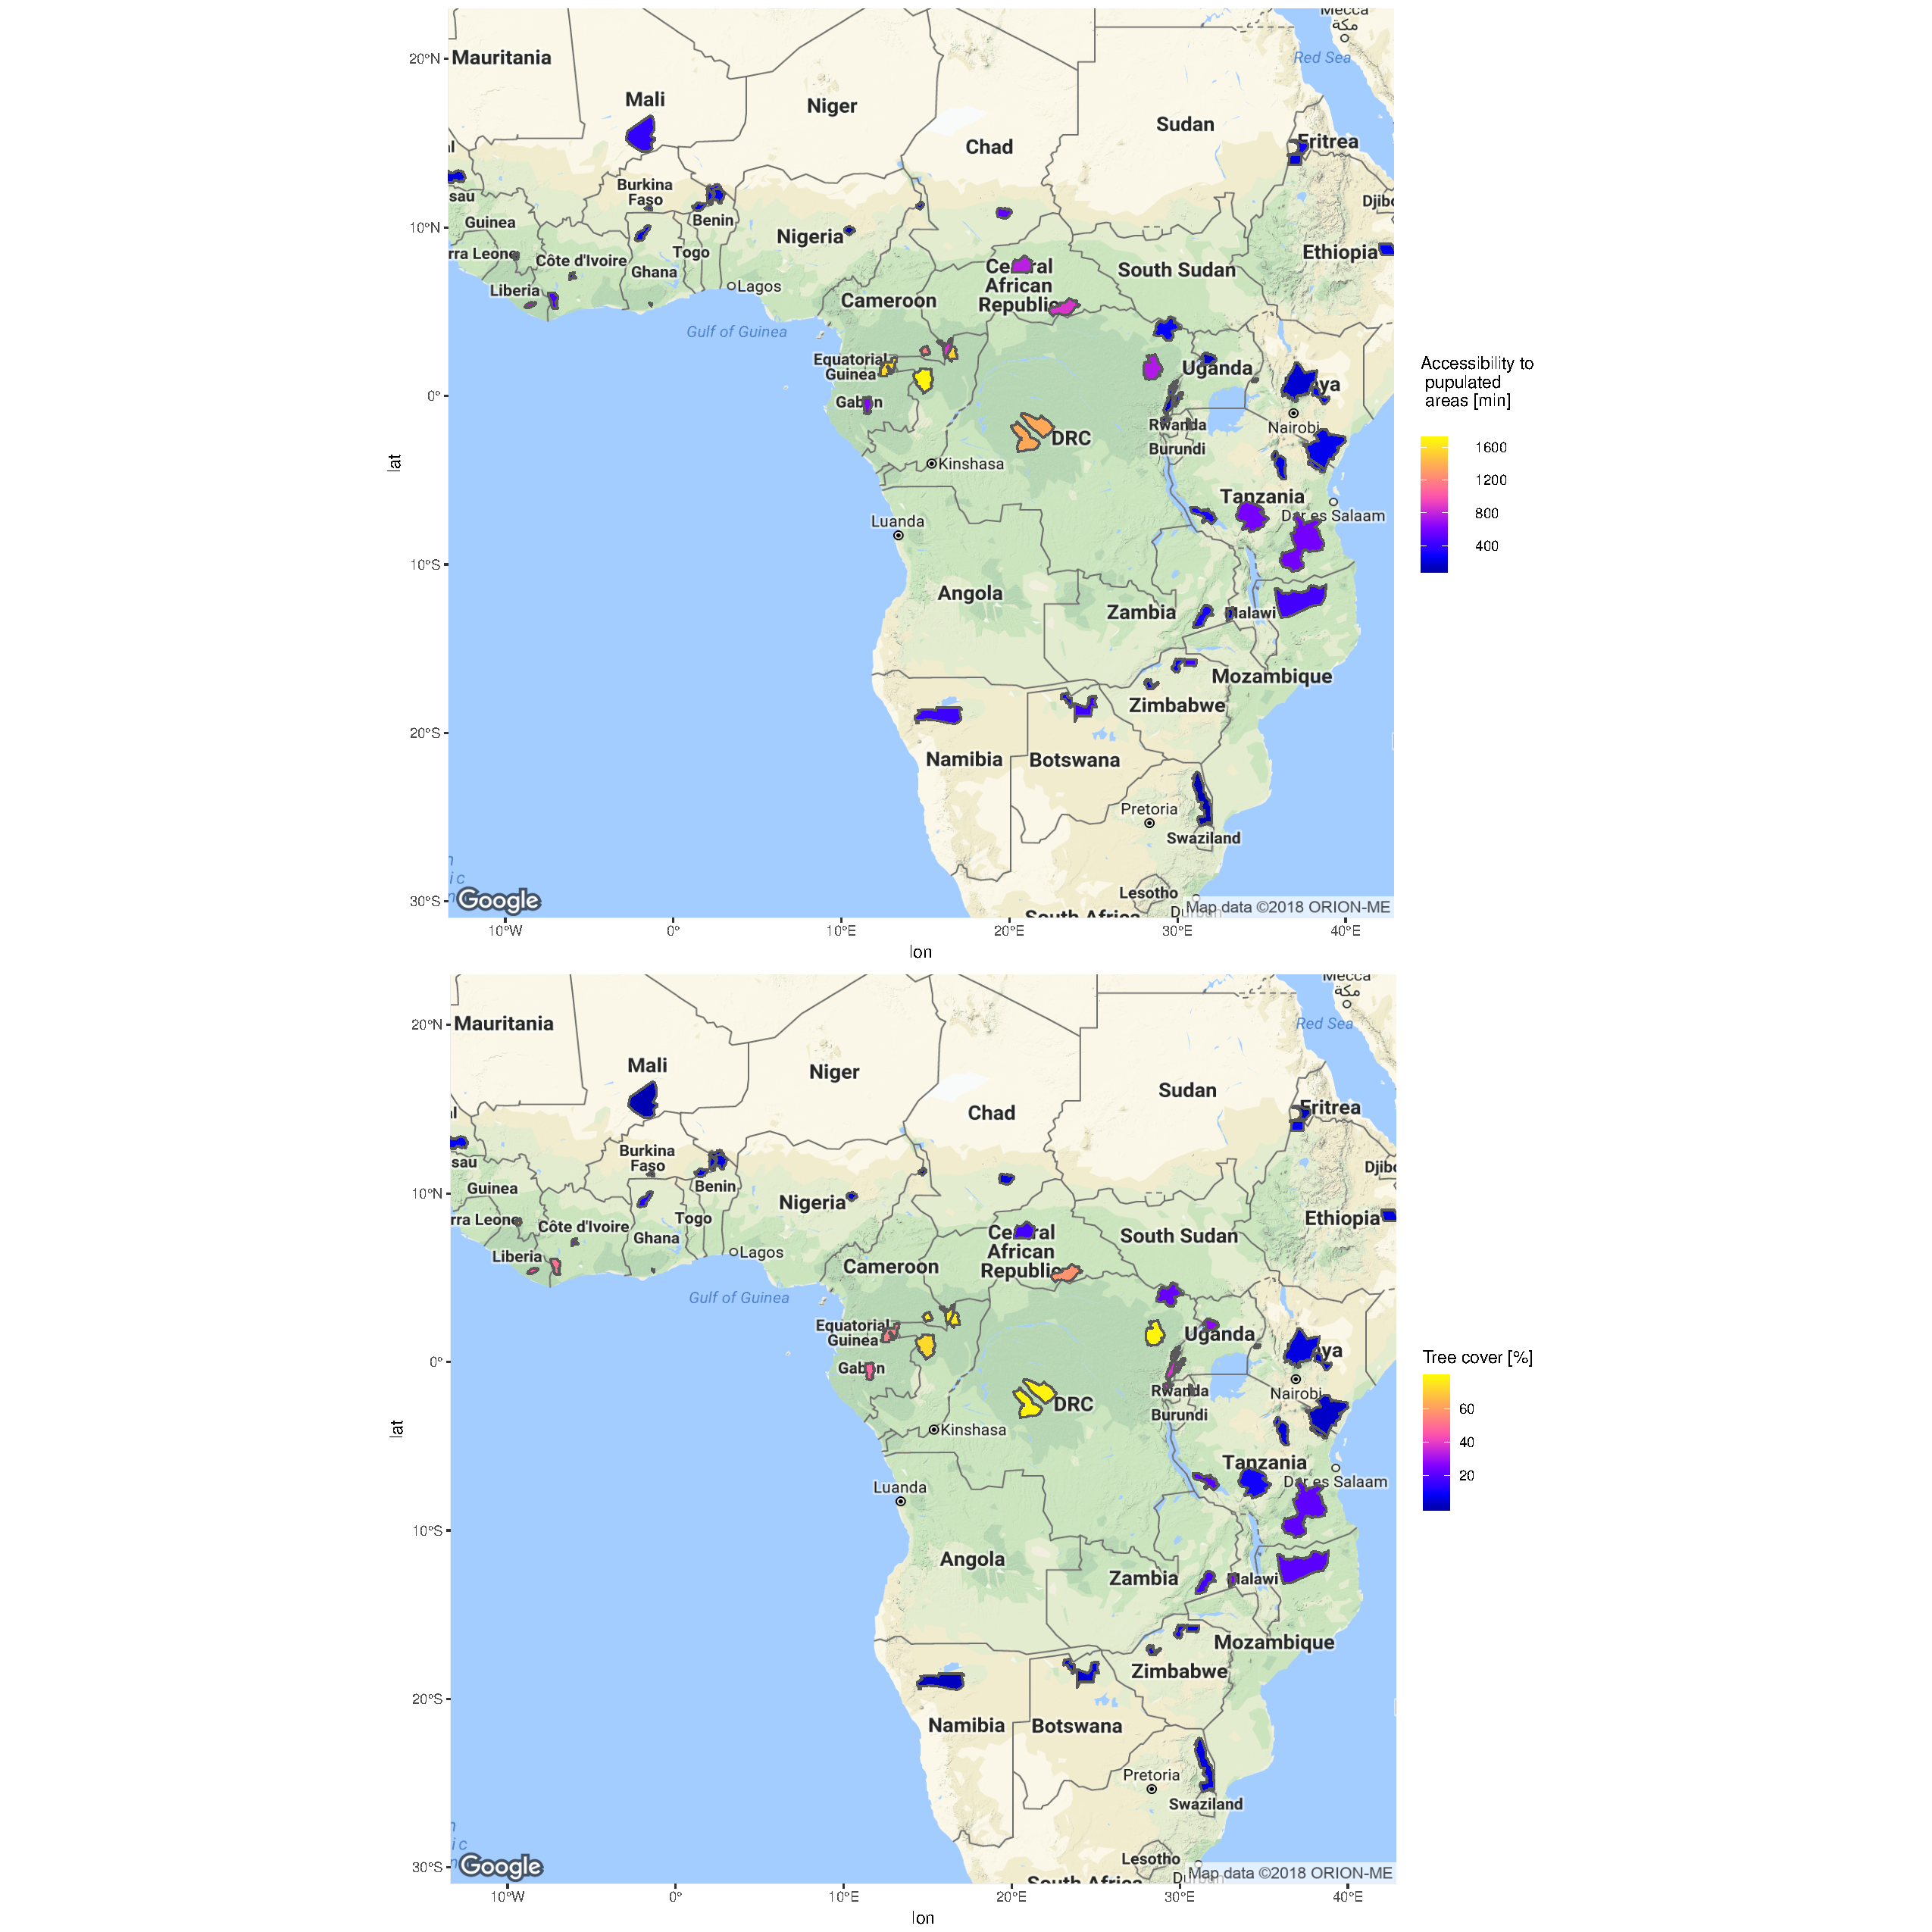
\includegraphics[width=15cm]{images/sample_session_1.pdf}
    \end{center}
  \end{figure}
 % \vskip 2em%
\end{center}

Map X shows the two data products. Eye-catching but not surprising is the negative correlation between accessibility and tree cover resulting in a regional pattern with the highest tree cover and lowest accessibility found in central Africa, while toward the north, south and west, the accessibility increases and the tree cover decreases.

While this sample session shows the capabilities of the earthEngineGrabR package to aggregate over large areas, the next example is dedicated to the opposite situation. 


\section{sample session 2}
\tableofcontents
let's stay with the invented scientist and his situation already described. Because of your access to the Great Elephant Census data you not only have the aggregated data for each territory but also the pre-aggregated survey data consisting of the number of elephants counted within a region specified by position, hight and the flight path of the aircraft. The combined regions form the spatial coverage of the survey and are available as shapefiles.

\begin{center}

   \begin{figure}[h]
     \begin{center}
       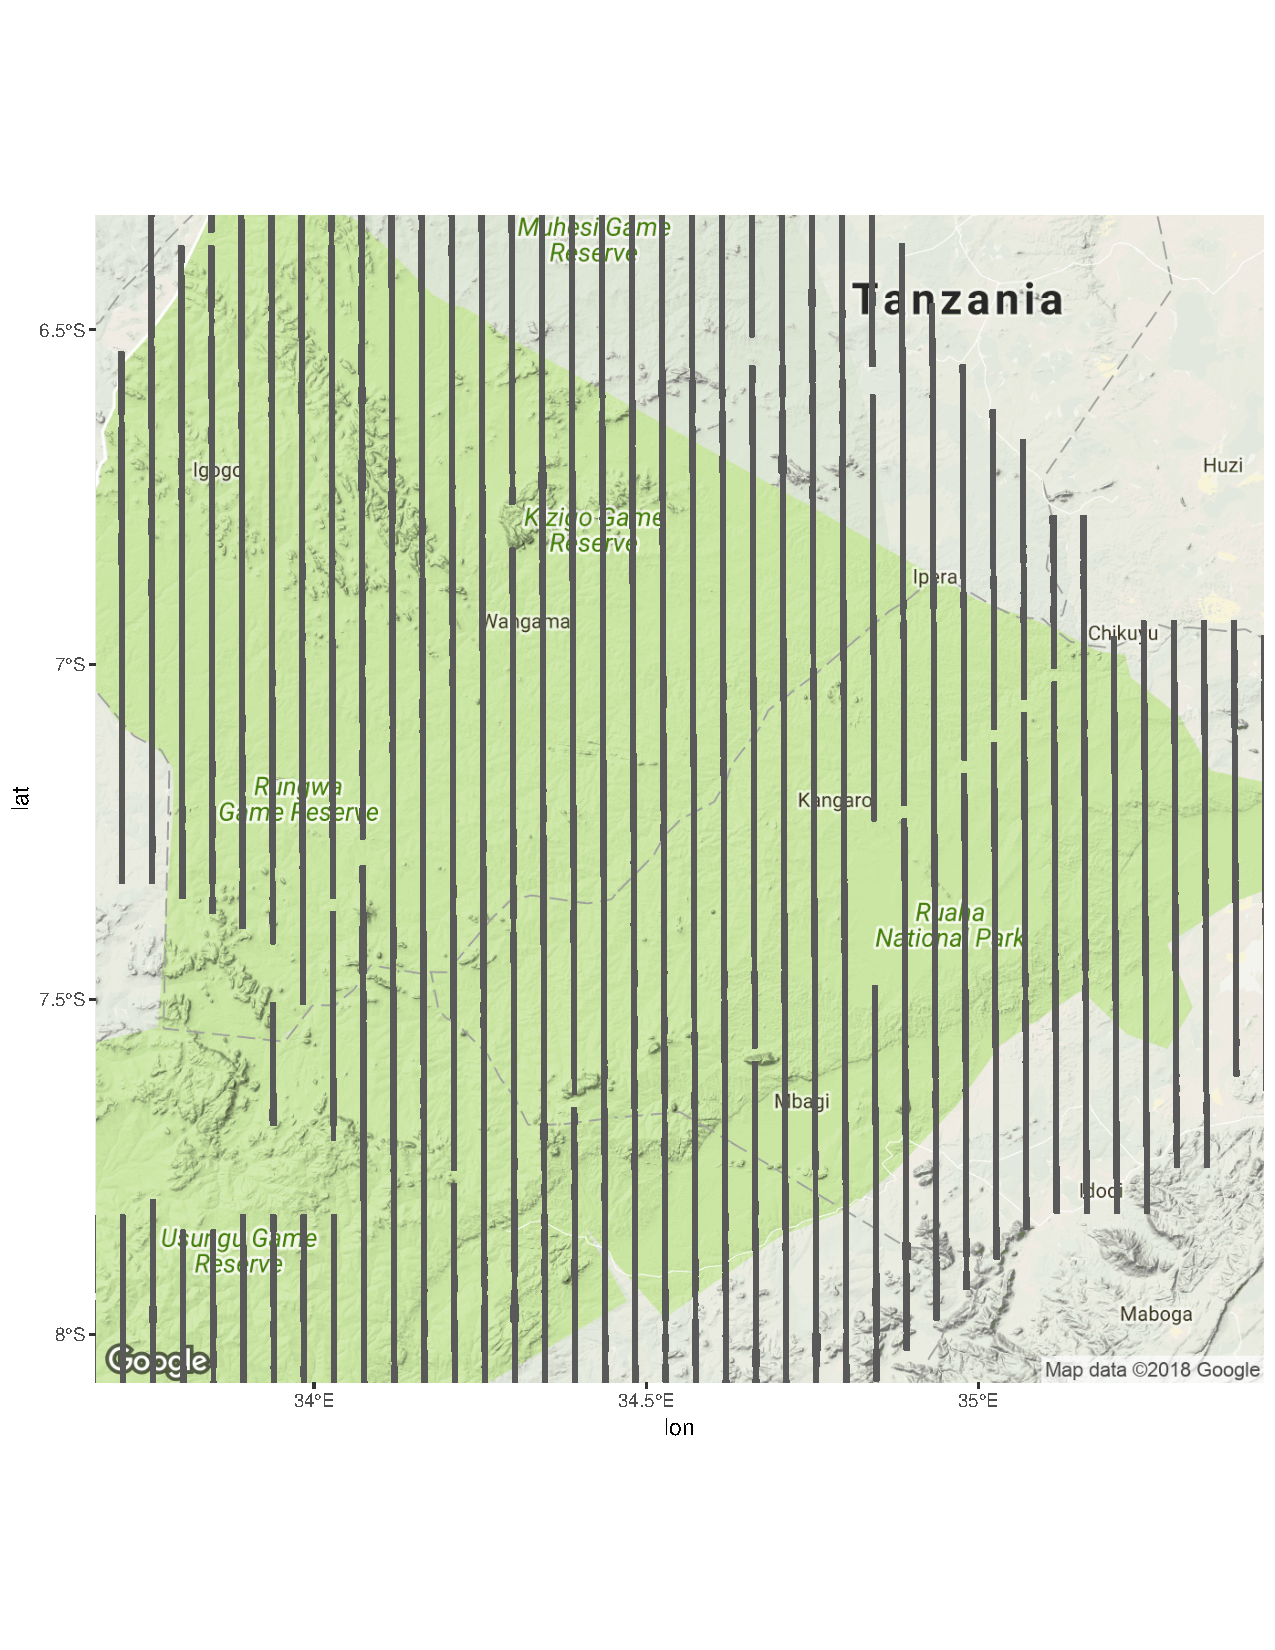
\includegraphics[width=15cm]{images/stripes.pdf}
    \end{center}
  \end{figure}
 % \vskip 2em%
\end{center}


Map X shows the coverage for Tanzania. This time you are interested in the availability of surface water in each of these regions, therefore you want to use the distance to surface water data product available in the earthEngineGrabR package. As the target, you use the shapefile of the survey coverage and only specify the \texttt{jrc\_distanceToWater} product in the products argument. As spatial and temporal reducer you choose median. 

\begin{lstlisting}

africa_elephant_data_stripes <- ee_grab(
  target = "../Data/Strips_shapefiles/RR16StripsAlignedForFig.shp", 
  products = list(
    eeProduct_jrc_distanceToWater(yearIntervall = c(2000,2000), spatialReducer = "median")
    ),
  resolution = 100
)
\end{lstlisting}




Due to the smaller area of the features of the target (mean area of 0.7 square kilometre), you choose a resolution of 50 meters and execute the function. The computation time takes about 3 minutes and the result is shown in map .y Since the area of the coverage is too small for a meaningful visualisation, map X shows a strongly zoomed view of the actual map x. 

\begin{center}

   \begin{figure}[h]
     \begin{center}
       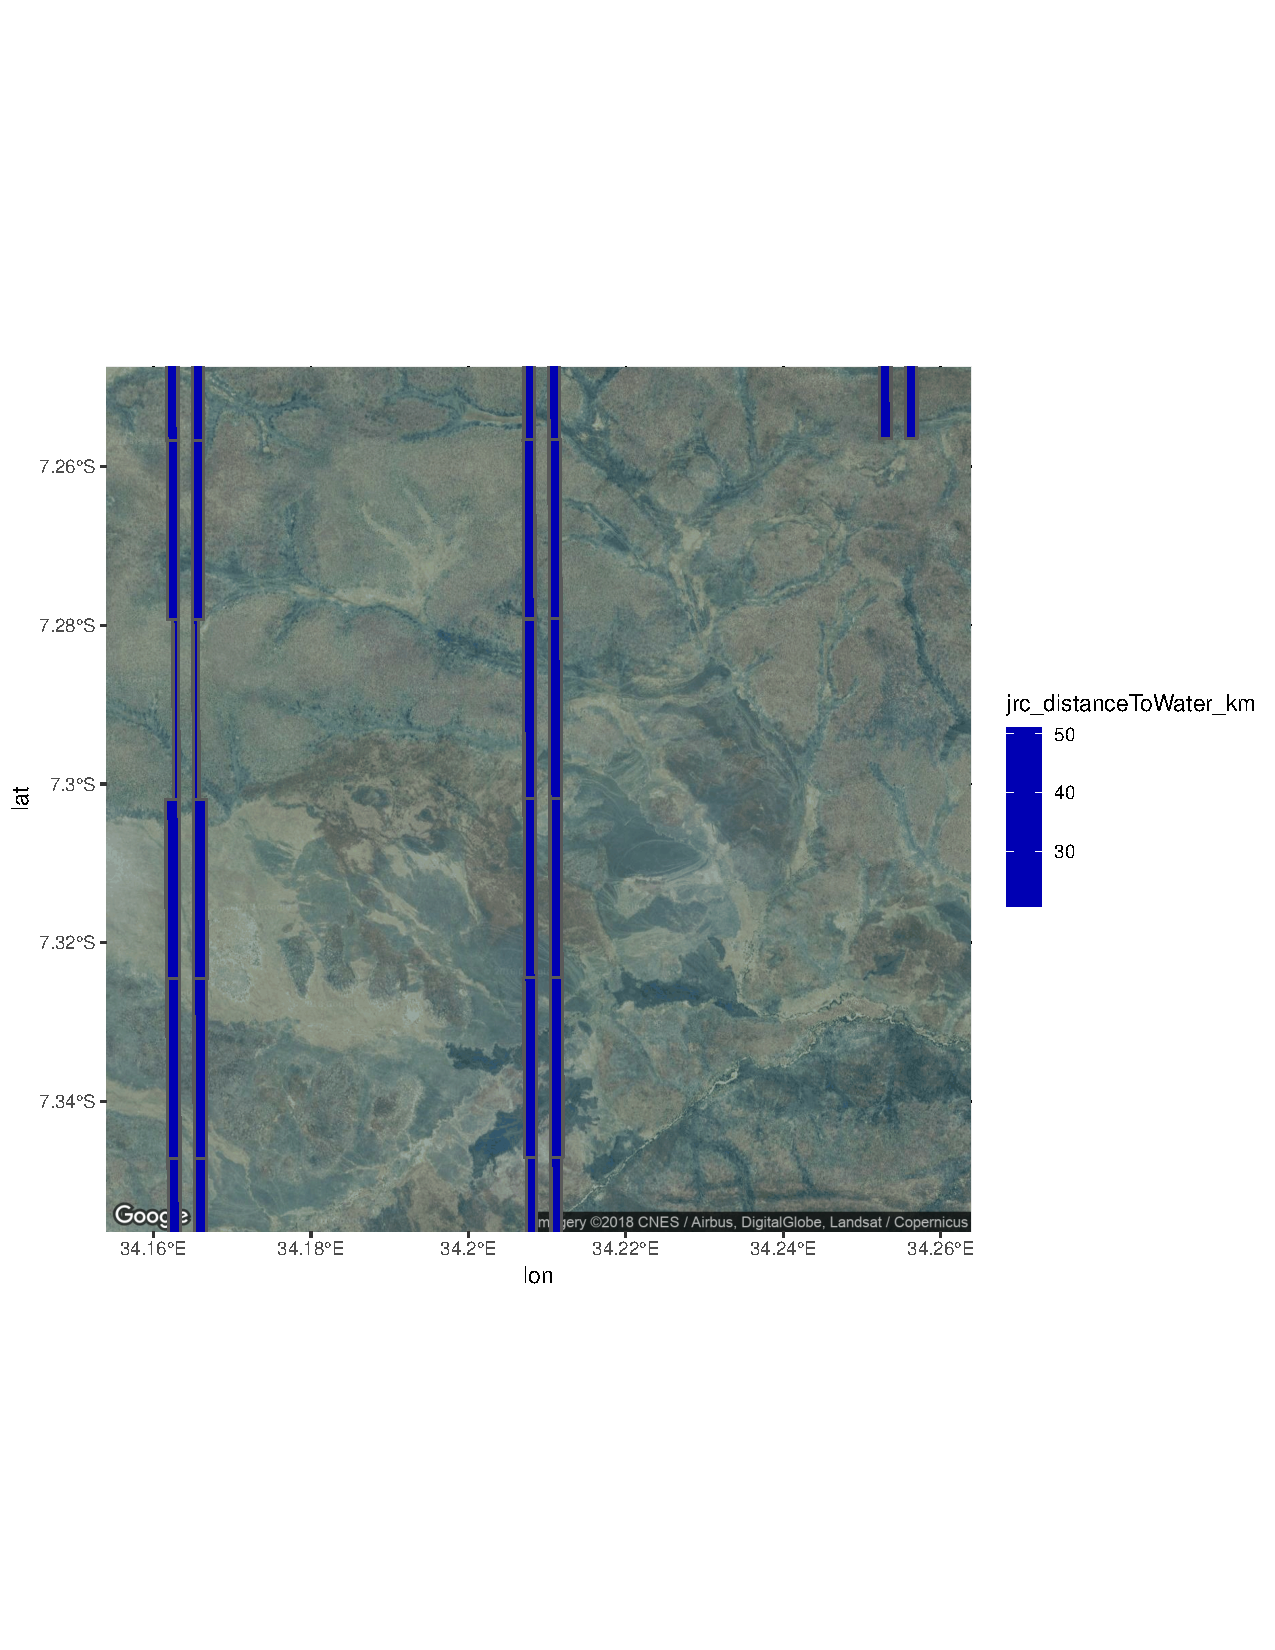
\includegraphics[width=15cm]{images/stripes_distance_zoom.pdf}
    \end{center}
  \end{figure}
 % \vskip 2em%
\end{center}



This example shows the flexibility of the earthEngineGrabR referred to the scale of analysis and the shape of the target.

In the last example, a more extended use case of the \texttt{ee\_grab} function is presented.


\section{sample session 3}

As a scientist, you are also interested in changes over time, for example, the change of precipitation in the elephant territories. Out of the documentation you know, that the precipitation product of the earthEngineGrabR is available from 2000 to 2015 on a yearly basis, thus you decide to calculate the precipitation for each year from 2000 to 2015 and analyse the change by using a linear model. The chirps precipitation product is produced from satellite data on a daily basis, what offers the possibility to calculate the yearly precipitation sum. Because the yearly precipitation sum is a common practice in hydrology and compared to the mean not this prone to extreme values you decide to calculate the yearly sum in each of the elephant territories for each year. To achieve that, you simply use the \texttt{ee\_grab} function, iterate over each year and collect the iteration products as follows:

\begin{lstlisting}

years <- 2000:2015
# empty data.frame for iteration
precipitation_all_years <- data.frame("name" <- NULL,"chirps_precipitation_mm" <- NULL, "year" <- NULL)

for (i in years) {
  # to inform
  cut(paste("processing of year:", i))
  # grab precipitation for year = i
  precipitation_year <- ee_grab(
    target = "../Data/drought_sites/mike_bnd_af.shp",
    products = list(
      eeProduct_chirps_precipitation(yearIntervall = c(i, i), temporalReducer = "sum")
    ),
    resolution = 1000
  )
  # to drop geometry, select variables of interest and creat a year column
  precipitation_year_clean <- precipitation_year %>% 
    sf::st_set_geometry(NULL) %>% 
    dplyr::select(chirps_precipitation_mm, name) %>% 
    dplyr::mutate(year = i)
  # accumulate iteration products
  precipitation_all_years <- dplyr::bind_rows(precipitation_all_years, precipitation_year_clean)
}
\end{lstlisting}




As temporal reducer, you choose sum, for the year interval, you take the i-th value of the created years vector. Due to the large-scale of your analysis, you again choose a resolution of 1000 meters. Since you want the spatial mean of the yearly precipitation sum in the territories, which already is the default spatial reducer, all necessary parameters in the \texttt{ee\_grab} function are specified. While the processing of a single request for one year would take about 3 minutes, the processing time of the entire for loop is only about 15 minutes. Because the requests are sent and processed in parallel, the relationship of the processing time and the number of requests is nonlinear. This point will be explained further in the discussion. The output of this loop is data.frame with a column for the sum of precipitation, year and name of the territory.  To quickly calculate, a linear model of the sum of precipitation explained by year for each of the territories you use a combination of functions from the dplyr and broom R packages. With dplyr's \texttt{group\_by} and do function you calculate a linear model for each of the territories and with the tidy function from broom and some selecting and filtering you extract the wanted estimates. The estimates show the linear effect of year on the yearly precipitation sum for each of the territories. 
By joining the estimates with the spatial data of the territories the estimates can be visualised spatially. 

\begin{center}
   \begin{figure}[h]
     \begin{center}
       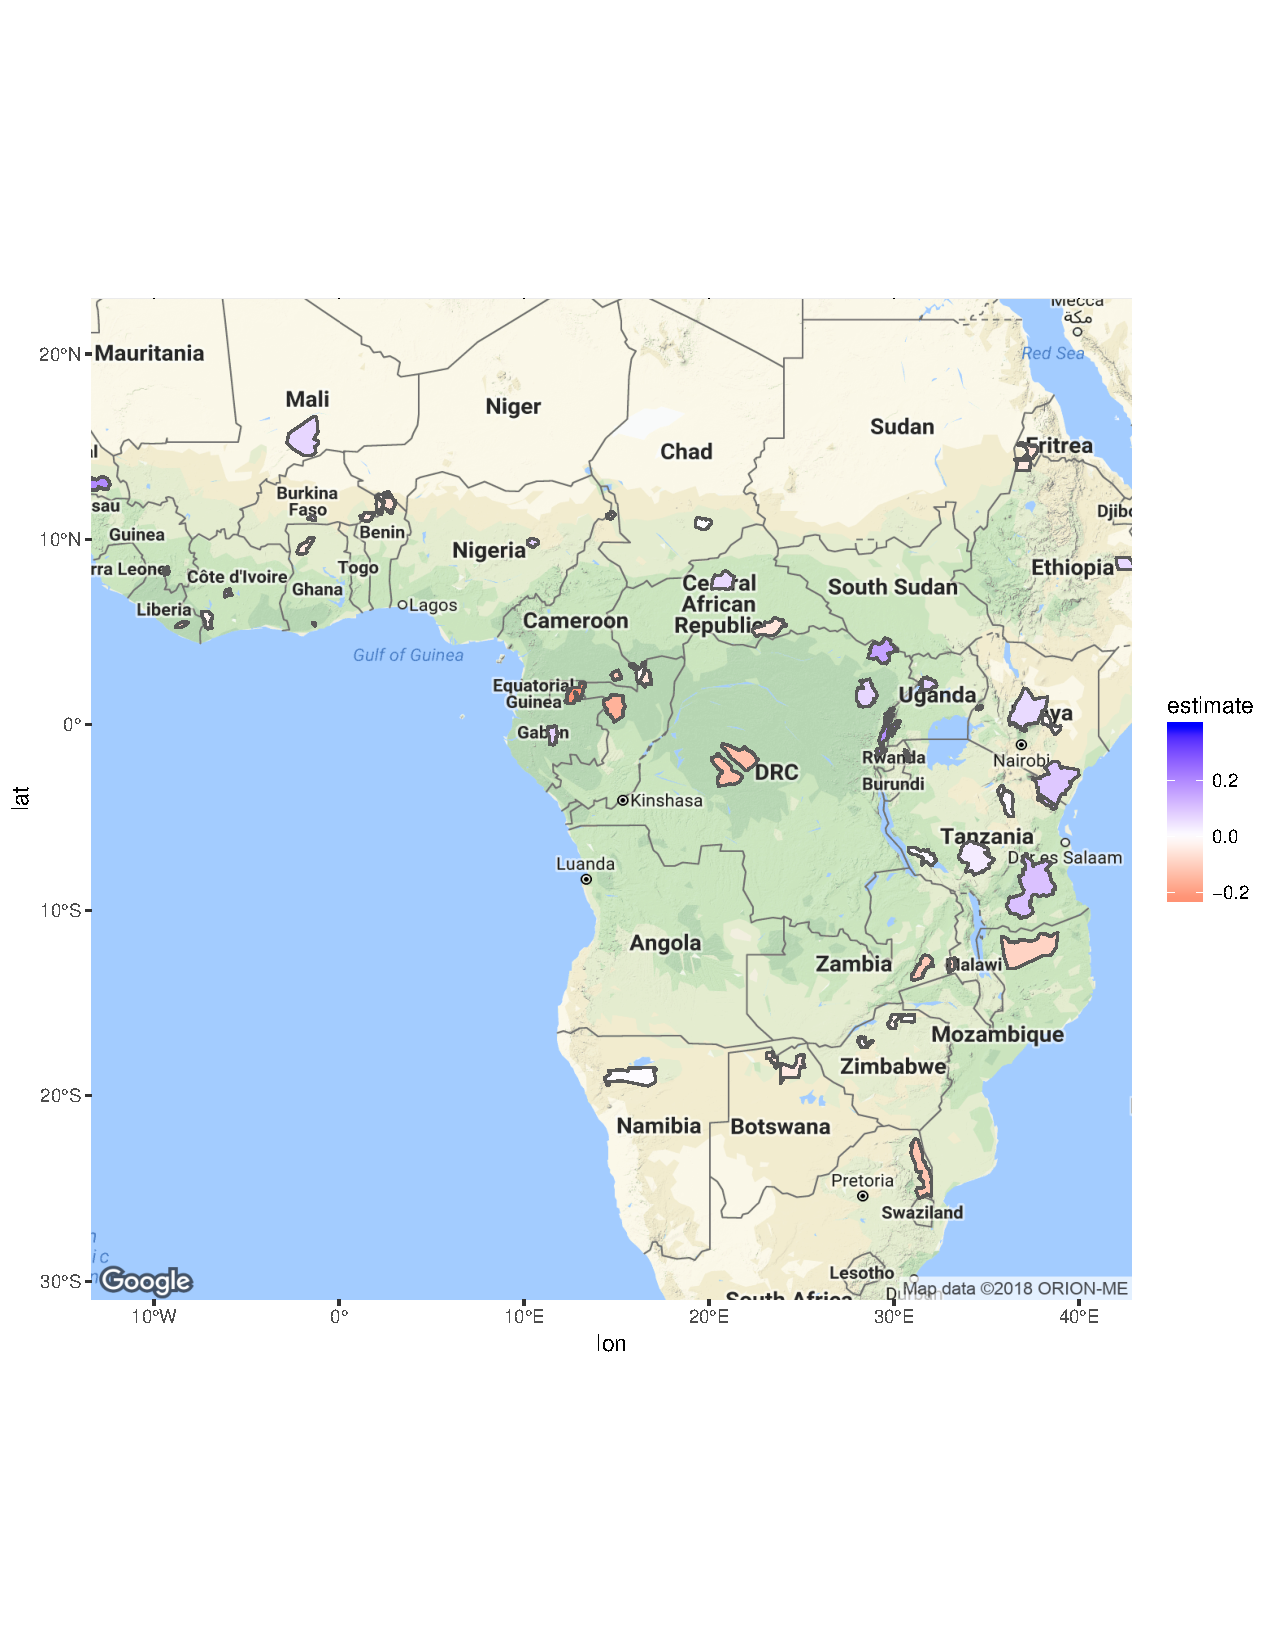
\includegraphics[width=15cm]{images/sample_session_3_change_map.pdf}
    \end{center}
  \end{figure}
 % \vskip 2em%
\end{center}



MapX shows the estimate of the yearly change of the yearly precipitation sum in for each territory. Given, that those estimates reflect a yearly change some values are remarkable hight. While the yearly precipitation sum is increasing for the territories in East Africa, it is decreasing for most territories in central Africa, especially for those with hight tree cover (see map X).


\chapter{Discussion}


The previous sample sessions in the results section showed the ability of the earthEngineGrabR to acquire remote sensing data for various research questions.
Compared to the traditional method described in the introduction the earthEngineGrabR is superior in various ways:
The use of the earthEngineGrabR to acquire remote sensing data for a specific time, region and aggregation provide significant savings of time, processing resources and labour. To acquire, the data for the research questions was a matter of minutes, even the aggregation of daily precipitation satellite imagery for 15 years took less than 15 minutes. The required processing resources for the computation was completely outsourced, while there was only a minimum of load on the local processing resources. Further, no manual preprocessing or integration of different data sources was necessary and no external GIS software had to be used. The entire process could be controlled from within R and only a minimum of GIS knowlege and no experience with Python or the earth engine Python API was recquired. With the earthEngineGrabR, the user not only could harvest data products from the earth engine data catalogue but with the aggregation process controlled by the user, could generate new data dependent on the research questions. 
Therefore, for the described use cased, it can be said, that the earthEngineGrabR strongly simplyfied and at the same time extended the possibility of the user to acquire remote sensing data for there research questions.
Thereby, the package shows the potential of a simplified access to the capabilities of the GEE for the scientific work.

\section{limits and problems of the current version of the earthEngineGrabR}

Although in some cases, the use of the earthEngineGrabR package offers some significant advantages to the scientific work, the current version is still limited in many ways. 

\subsubsection{small file size of vector data}

Particularly, due to the current upload limit of the fusion table API, it's not possible to process vector data with more than 5000 features. This small size certainly restricts the application of the package and would make it uncomely for most scientific projects. 
 
\subsubsection{a limited number of available data products and their possible properties}

Furthermore, the choice of available data products and their properties in the earthEngineGrabR is still low. The package, for example, offers no product for temperature, climate or any vegetation indexes and the available products lack a necessary temporal resolution. For instance, since the smallest temporal interval is one year, it's not possible to request the precipitation or distance to surface water for a certain season. But for the most ecological problems, the seasonality is of great importance.


\subsubsection{no projection control}

Another problem that is unsolved yet, is that during the upload process all vector data is transformed to geographic reference system WGS84. That is, that all the processing in earth engine is performed without a projection unless you call the WGS84 a projection. Therefore all projections of the original vector data are lost. The output of the \texttt{ee\_grab} function does not reflect the projection of the imported vector data. The conversion to WGS84 is unproblematic as long as there is no calculation of areas. Since the spatial reducer of the earthEngineGrabR only allows simple statistics like mean, median, mode, min and max, there is no calculation of areas and the conversion to WGS84 is harmless to the results of the analysis. However, in most cases, it would require a manual reprojection of the results by the user to combine the data collected by the earthEngineGrabR with data that is already at hand. An additional control of the projection would be helpful.

\subsubsection{challenge to get all dependencies to work, different operating systems, the confusing authentication process}
 

The most challenging problem though is to get the earthEngineGrabR to work on all operating systems properly. This point is challenging because of the many requirements and dependencies of the package. There are dependencies to R packages python libraries and external libraries like GDAL and there has to be a working python distribution on the system with a specified python path as an environmental variable. An additional difficulty is the confusing and extensive authentication process. While the Google Drive and Fusion Table API are accessed directly with R, the earth engine API and the gdal driver for fusion tables are accessed with python. In R the authentication protocol is managed by the httr R package and requires no manual copying and pasting of authorisation tokens. For the authorisation to the API's accessed from python the copy and pasting of tokens are still necessary. 
Furthermore, the httr R package in its current implementation of the earthEngineGrabR works with access tokens, which need to be refreshed after approximately an hour while the authentication protocols managed with different python libraries work with refresh tokens, which never expire and therefore only need one initial authorisation. While using the earthEngineGrabR, this results in regular interruptions where the user is asked to again log in to his Google Account. Although with an already logged in account, this is simply one click with a mouse per hour, this can be problematic for unsupervised use of the package for instance on a  server. Therefore, although already strongly simplified, the current management of the dependencies and authentication protocols is still error-prone and requires too much activity on the user's side.

\section{future work and further enhancements}

Most of the shortcomings addressed in the last section can be rectified with the further development of the earthEngineGrabR package. As mentioned in the methods section, the current version of the package is supposed to provide a stable framework for the base functionality of the package like: 

\begin{itemize}

\item uploading data to earth engine
\item select a data product
\item rovide extensive control over the aggregation corresponding to the shape, temporal and spatial resolution
\item export data products from earth engine and import the products into R
\item manage the dependencies and authorisations to the involved API's

\end{itemize}



The further development can be divided into the improvement of the framework and the implementation and the further development of additional features.
Below, a number of additional extensions to the earthEngineGrabR is described that would rectify most of the addressed shortcomings.


The most urgent extension is the implementation of additional data products. Basically, all data products available within the Earth Engine public data catalogue can be considered (In the appendix, table n. gorelick, list of the available datasets). Ath the moment the implementations are driven by demand. To provide data products covering weather and climate conditions, the implementation of additional products based on ASTER (Advanced Spaceborne Thermal Emission and Reflection Radiometer) and MODIS would be reasonable. Furthermore, a data product to provide vegetation indices calculated form Sentinel or Landsat satellite imagery would be exciting. This product, for example, would provide to choose a time interval in months, maximum cloud cover to filter the image collection, whether to use Landsat or Sentinel imagery to calculate the Index and a selection of possible vegetation indexes like the NDVI (Normalized Difference Vegetation Index) or NDBI (Normalized Difference Built-up Index) etc. 

\subsubsection{if available allow a monthly resolution}
 

In addition, the available data products in the earthEngineGrabR: the chirps precipitation products and jrc distance to surface water product, receive a monthly resolution. In the time interval argument, this would result in the possibility to specify year and month of the interval of interest.

\subsubsection{control the spatial resolution for each product separately}
 



Furthermore, it would be reasonable to choose the spatial resolution for each data product separately and add control over the projection of the analysis. 


\subsubsection{add more control of projections}
 
 
This could be achieved by simply taking the target projection and send it as a string that specifies the EPSG (European Petroleum Survey Group - list of codes for geographic reference systems) to the earth engine servers and reprojects the requested data. Another option would be to control the projection explicitly with an additional argument.

\subsubsection{add internal iterations to increase the number of possible features to be processed}


it would require a manual subdivision and partial processing of the vector data what is 

To increase the overall file size and the number of features of the target that can be processed it's necessary to build a workaround for two internal limitations of the Earth Engine API and the Fusion Table API. One is the upload limit for Fusion Tables, of around 5000 features at a time and another an export limit of Earth Engine of about 70 000 features at a time to Google Drive. The workaround for both limitations is to subdivide the file, iterate over the request of each subdivision and finally merge the subdivision results back together. This could be done in the following way: In the Fusion Table API, it's possible to upload vector data as a new Fusion Table or add to an existing one. Therefore, in the beginning, the file could be subdivided into chunks, that don't exceed 5000 features. While the first chunk is used to upload a new Fusion Table all additional chunks can be added in an iteration process. This existing Fusion Table is used as the target in Earth Engine. If the export exceeds 70 000 features it is again subdivided into multiple requests, downloaded separately and merged during the import process in R. This approach would enable the processing of considerably larger vector data and furthermore make use of a performance gain achieved by parallelisation and iteration. This effect was already mentioned in the last sample session example in the results section and will be pointed out in the following tips and tricks section.

\subsubsection{change the authentication process so that no manually copy or pasting is necessary anymore}



To simplify the authentication process it would be relevant to replace the manually copy and pasting of the authorisation tokens with an automatic transfer. Next, all authorisation processes should work with a refresh token which only requires one initial authorisation. The produced credentials refresh automatically without the intervention of the user. To further shield the user from the authorisation process it would be reasonable to incorporate the \texttt{ee\_grab\_init} inside the \texttt{ee\_grab} function and run the initialisation if the credentials cannot be found. This way, if the user calls the \texttt{ee\_grab} function the first time, \texttt{ee\_grab\_init} gets called and triggers the authorisation process. 


\subsubsection{possibility for the user to add and define new data products}


Finally, it would be necessary to consider a possibility to add new data products by the user himself. To achieve this either the earthEngineGrabR has to provide a function that works with all datasets on the Earth Engine Data Catalog or there is detailed documentation on how to create your own data products and the user acts like a coworker that incorporate changes to the earthEngineGrabR using the version control system of GitHub. This two examples certainly are extremes of two different designs of the earthEngineGrabR and a solution should make use of both directions. In the broader sense, it's the question of how to provide extensibility to the users. It seems necessary that demanded features are implemented by the package maintainer. However, to supply tools, that the users can build the required data products himself is probably superior to one individual being responsible for the implementation of every request.
Independently of the different approaches of how to provide extensibility, there are several implementations that would certainly simplify the integration of additional features and the collaboration with other users of the earthEngineGrabR package. The first is, to provide a comprehensive documentation with additional sample sessions, vignettes or tutorials. Next, to implement tests in the development workflow and use them for Continuous Integration (CI). Discarding, of the improved stability of the package, testing and CI would improve the collaboration with co-workers and simplify the publication of the earthEngineGrabR. 

To improve the framework for the base functionality of the earthEngineGrabR package the interface of R and Python could be changed. Instead of an interface depending on the console which invoiced system calls in the way described in the methods section the new published reticulate package for r-studio could be used. The use of reticulate would offer some significant benefits. The reticulate package offers the translation of R and Python data types. This would overdue the use of a flat file connection to pass parameters or processing info. Further, retuculate contains a multitude of helper functions that ease the use of R in combination with Python (\texttt{py\_available()}, for instance, checks for a python version on the system). While the execution of pythons scripts with a console, require the python code organised as scripts, with reticulate it's possible to run python code directly in R and organise the code in smaler, more flexible chunks, what is important when it comes to tools that provide the option to expand the earthEngineGrabR with additional data products and functionalities. The use of the reticulate package also would simplify the installation of python dependencies, because they can be performed in R (\texttt{py\_install()}- installs python libraries).
In summary, the reticulate package would provide a more precise, less error-prone and more flexible interface of R and Python then the currently implemented use of system calls.

\section{Internal limitations of the GEE and what this implies for the earthEngineGrabR}

Besides the discussed limitation, there are also limitations of the GEE, that in contrast to the limitations of the earthEngineGrabR, can't be avoided by further development of the package. These internal limitations have a strong influence on the operations that can be performed with the package. 

\subsection{Limitation of processing resources}


\subsubsection{System throughput an performance}

A reason for Earth Engines performance is its ability to efficiently distribute and manage complex computations across many machines. There is an almost linear relationship of throughput (pixels/sec) with the number of machines.
Although the Earth Engine can execute and manage extremely large computations, the underlying infrastructure consists of clusters of low-end servers and there is a hard limit on the amount of data that can be brought into any individual server. The current Remote procedure call (RPC) and caching system limit the size of an object to 100 MB.
An option to configure machines in earth engine is not available.
Users can only express computations by using the parallel processing primitives provided in the Earth Engine client library and some non-parallelizable operations simply cannot be performed effectively in this environment.
During the development of the earthEngineGrabR, the experience was repeatedly made, that requests of smaller magnitude are processed fast and immediately while requests exceeding a certain magnitude in data throughput, result in unforeseeable long data processing. Unfortunately, due to the reason, that the Earth Engine system hides nearly every aspect of the computation from the user, the magnitude generating this bottleneck is not obvious. Hence, avoiding the bottleneck saves hours of computation time and also enables processes that otherwise result in errors referring to computation timeout or user memory limit exceeding. For example, processing all available data products and joining them in one request, given a target shapefile of 10.000 features, takes more than 1 hour of computation, while iterating over the data products with one request each, is a matter of a few minutes. This insight is reflected in the internal design of the earthEnigneGrabR. In the \texttt{ee\_grab} function, each data product is processed individually. Furthermore, this approach allows processing the data products in parallel. The individual requests for the data products, generated by the GEE client library in python, all end with a command to export the generated data to Google Drive. However, the request must not wait until the data is processed. Instead, the request ends with the response of the earth engine servers, whether earth engine started a valid export or not. Yet, on the server side, the start of the export is the moment the actual computation of the data is initialised. This allows requesting the computation of multiple data products at the same time. The exported data products are individually downloaded from Google Drive and joined in R. This way, data bottlenecks, resulting in long export and computation timeout errors are avoided. 
In summary, the performance of the earthEngineGrabR depends on earth engines ability to efficiently distribute computation by an internal parallelisation mechanism, that can't be controlled by the user. Operations that can't be efficiently scaled result in unforeseeable long processes and error and slow down the computation. By dividing requests with high data throughput in multiple smaller request, this internal limitation partly is avoided.

\subsubsection{Export limitation}

The GEE provides data export to Google Drive and Google Cloud Platform (GCP). While the export to GCP is fast and works with very large datasets, the export to Google Drive is limited to 2 GB and proportionally slow. Due to the reason, that outside the USA the always free tier of the GCP is not available, the export to Google Drive is the only free option. Similar to the described data bottleneck, discarding the official limit of 2 GB, it has shown that keeping the size of the export smal dramatically speeds up the process while export files larger 200 MB can result in hours of computation time. While this limitation can partly be avoided by the iteration approach described, it strongly restricts the download of large files.



%\chapter*{Acknowledgements}

\label{ch:Acknowledgements}
\addcontentsline{toc}{chapter}{Acknowledgements}


Firstly, I would like to express my gratitude to my advisor Severin Hauenstein for the continuous support of this thesis, for his patience and motivation. His commitment helped and inspired me throughout the time of the thesis.

My thanks also go to my co-supervisor Mirko Mälicke who gave me vital technical support at the beginning.

Besides my advisors, I would like to thank Prof. Dr Carsten Dormann, for his encouragement during the thesis and especially for his time in many little and precious talks before. 
I further want to thank Dr.-Ing. Holger Weinacker who immediately agreed to be the second reader.

I want to thank my dear friends and companions in misfortune and happiness Simon and Samuel for there sympathy, knowledge and friendship.
Finally, I very much thank Julia Angstenberger for her strong and brave proofreading.

Last but not least, I want to thank my wonderful girlfriend Katharina for her understanding and caring support and apologise for all hours of tiredness, despair and inattention.









\printbibliography


% Insert the first appendix
\chapter{This is Appendix 1...}
\label{app:appendix1}

Put appendix text here


% Insert the second appendix

% insert a second appendix
\chapter{Appendix}
\label{app:appendix2}


\begin{table}[h]
	\tiny
	\begin{tabularx}{\textwidth}{lXXXX}
		\toprule
		\textbf{Dataset} & \textbf{Nominal resolution} & \textbf{Temporal granularity}  & \textbf{Temporal coverage}  & \textbf{Spatial coveragee} \\
		\hline
		Landsat & & & & \\
			Landsat 8 OLI/TIRS	&30 m	&16 day&	2013–Now&	Global\\
			Landsat 7 ETM +	&30 m	&16 day	&2000–Now&	Global\\
			Landsat 5 TM	&30 m	&16 day	&1984–2012&	Global\\
			Landsat 4–8 surface reflectance	&30 m	&16 day	& 1984–Now &	Global\\
		Sentinel & & & & \\        
		Sentinel 1 A/B  &10 m	&6 day	&2014–Now	&Global \\
		Sentinel 2A MSI  &10/20 m	&10 day&	2015–Now&	Global\\
		
		MODIS & & & & \\  
		
		  MOD08 atmosphere&	$1^\circ$ &	Daily	&2000–Now&	Global\\
		  MOD09 surface reflectance&	500 m&	1 day/8 day&	2000–Now&	Global\\
		  MOD10 snow cover&	500 m&	1 day&	2000–Now&	Global \\
		  MOD11 temperature and emissivity&	1000 m&	1 day/8 day&	2000–Now&	Global\\
		  MCD12 Land cover&	500 m	&Annual	&2000–Now	&Global \\
		  MOD13 Vegetation indices&	500/250 m	&16 day	&2000–Now&	Global\\
		  MOD14 Thermal anomalies  fire&	1000 m&	8 day&	2000–Now&	Global\\
		  MCD15 Leaf area index/FPAR&	500 m&	4 day&	2000–Now&	Global\\
		  MOD17 Gross primary productivity	&500 m&	8 day&	2000–Now&	Global\\
		  MCD43 BRDF-adjusted reflectance	&1000/500 m&	8 day/16 day&	2000–Now&	Global\\
		  MOD44 veg. cover conversion&	250 m&	Annual&	2000–Now&	Global\\
		  MCD45 thermal anomalies and fire	&500 m&	30 day&	2000–Now&	Global\\
		
		 ASTER	& & & & \\	
		 L1 T radiance	&15/30/90 m	&1 day&	2000–Now&	Global \\
		 Global emissivity	&100 m	&Once	&2000–2010&	Global \\
		  
		 Other imagery	& & & & \\		
		 PROBA-V top of canopy reflectance&	100/300 m&	2 day&	2013–Now&	Global\\
		 EO-1 hyperion hyperspectral radiance&	30 m&	Targeted&	2001–Now&	Global\\
		 DMSP-OLS nighttime lights&	1 km&	Annual&	1992–2013&	Global\\
		 USDA NAIP aerial imagery&	1 m	&Sub-annual	&2003–2015& 	CONUS\\
		 
		 Topography			& & & & \\		
		 Shuttle Radar Topography Mission&	30 m&	Single&	2000&	$60^\circ$ N–$54^\circ$ S\\
		 USGS National Elevation Dataset&	10 m&	Single&	Multiple&	United States\\
		 USGS GMTED2010&	$7.5''$&	Single	&Multiple&	$83^\circ$ N–$57^\circ$S\\
		 GTOPO30&	$30''$	&Single	&Multiple	&Global\\
		 ETOPO1	& $1'$ &	Single&	Multiple &	Global \\
		 
		 Landcover		& & & & \\			
		 GlobCover	&300 m	&Non-periodic	&2009&	90°N–65°S\\
		 USGS National Landcover Database&	30 m	&Non-periodic	&1992–2011&	CONUS\\
		 UMD global forest change&	30 m&	Annual	&2000–2014&	$80^\circ$ N–$57^\circ$ S\\
		 JRC global surface water&	30 m&	Monthly	&1984–2015	&$78^\circ$ N–$60^\circ$ S\\
		 GLCF tree cover&	30 m	&5 year	&2000–2010	&Global\\
		 USDA NASS cropland data layer&	30 m&	Annual&	1997–2015&	CONUS\\
		  
		 Weather, precipitation, atmosphere	& & & & \\				
		 Global precipitation measurement& 	$6'$& 	3 h	& 2014–Now& 	Global\\
		 TRMM 3B42 precipitation& 	$15'$& 	3 h	& 1998–2015	& $50^\circ$ N–$50^\circ$ S\\
		 CHIRPS precipitation& 	$3'$& 	5 day& 	1981–Now& 	$50^\circ$ N–$50^\circ$ S\\
		 NLDAS-2& 	$7.5'$& 	1 h	& 1979–Now	& North America\\
		 GLDAS-2& 	$15'$& 	3 h	& 1948–2010	& Global\\
		 NCEP reanalysis& 	$2.5^\circ$ & 	6 h	& 1948–Now& 	Global\\
		 ORNL DAYMET weather& 	1 km& 	Annual& 1980–Now& 	North America\\
		  
		 GRIDMET&	4 km&	1 day&	1979–Now&	CONUS\\
		 NCEP global forecast system&	$15'$&	6 h&	2015–Now&	Global\\
		 NCEP climate forecast system&	$12'$	&6 h&	1979–Now&	Global\\
		 WorldClim	&$3''$ &	12 images&	1960–1990&	Global\\
		 NEX downscaled climate projections&	1 km&	1 day&	1950–2099&	North America\\
		 Population		& & & & \\		
		 WorldPop	&100 m	&5 year	&Multiple	& 2010–2015\\
		 GPWv4	& $30''$ &	5 year&	2000–2020&	$85^\circ$ N–$60^\circ$ S\\
		\bottomrule
	\end{tabularx}
	\caption{Frequently used datasets in the earth engine data catalog (\cite{gorelick2017google})}
	\label{dependencies}
\end{table}



% If you used the makeidx package to create an index then use the 
% following command to print the index
\printindex

\chapter*{Selbstständigkeitserklärung} % (in German!)

\vspace{2cm}

\section*{Erklärung}

Ich versichere hiermit, dass ich die vorliegende Arbeit ohne fremde Hilfe selbstständig verfasst und nur die angegebenen Quellen und Hilfsmittel benutzt habe. Wörtlich oder dem Sinn nach aus anderen Werken entnommene Stellen habe ich unter Angabe der Quellen kenntlich gemacht.

\medskip
\noindent (I hereby declare that I have composed this document unassistedly and that I only used the sources and devices I declared. Passages taken verbatim or in meaning from other sources are identified as such and the sources are acknowledged and cited.)

\vspace{2cm}

\noindent \year

\end{document}